\documentclass[12pt,a4paper,tikz,border=5pt]{article}

\usepackage[utf8]{inputenc}
\usepackage[T1]{fontenc}
\usepackage{geometry}
\usepackage{enumitem}
\usepackage{xcolor}
\usepackage{mdframed}
\usepackage{parskip}
\usepackage{hyperref}
\usepackage{titlesec}
\usepackage{amsmath}
\usepackage{forest}
\usepackage{mathpartir}
\usepackage{tikz}
\usepackage{float}
\usepackage{listings}
\usepackage{booktabs}
\usetikzlibrary{automata,positioning}
\definecolor{grigiochiarissimo}{RGB}{245,245,245}

\geometry{margin=2.5cm}




\newcommand{\domanda}[3]{%
  % #1 = numero, #2 = testo domanda, #3 = risposta
  \subsubsection*{Domanda #1}
  \textbf{#2}
  \begin{mdframed}[backgroundcolor=grigiochiarissimo, linecolor=gray!50, linewidth=0.6pt, innertopmargin=6pt, innerbottommargin=12pt, innerleftmargin=8pt, innerrightmargin=8pt]
    \textit{#3}%
  \end{mdframed}%
  \vspace{0.4em}
}

\title{%
  \textbf{Domande per l'Orale LP}\\[0.4em]
  \large Modulo I/II/III%
}
\author{}
\date{}

\begin{document}

\maketitle


\tableofcontents
\newpage

% ================================================================
\section{Modulo 1 -- Gorrieri}
% ================================================================

% ----------------------------------------------------------------
\subsection{Capitolo 1 -- Macchine astratte, interpreti, compilatori}
% ----------------------------------------------------------------

\domanda{1}{Che cosa e una macchina astratta? E in cosa si differenzia da una macchina fisica?}{E' un insieme di algortimi e strutture dati che dato un programma scritto in un linguaggio relativo alla macchina astratta, quest'ultima lo esegue.\\
Una macchina fisica e' un insieme di circuiti logici composti da circuiti elettrici che allo stesso modo della macchina astratta dato un linguaggio specifico (conforme all'IS), la macchina fisica lo esegue.}

\domanda{2}{Che cos'e un interprete? In cosa consiste il ciclo fetch-decode-execute?}{Un interprete e' un programma che viene eseguito su un calcolatore che serve per eseguire in realtime un programma, senza prima doverlo compilare. Serve per poter eseguire un linguaggio $\mathcal{L}_A$ su un calcolatore che nativamente esegue il linguaggio $\mathcal{L}$. L'interprete eseegue il codice leggendo una istruzione alla volta.\\
FDE e' lo schema della CPU nel quale prende, decodifica ed esegue una istruzione. Questo e' fortemente collegato alla pipeline della CPU.}

\domanda{3}{Cos'e il linguaggio macchina?}{E' linguaggio relativo all'interprete $I_\mathcal{L}$ per la macchina $M_\mathcal{L}$.}

\domanda{4}{Possono esistere macchine diverse con lo stesso linguaggio macchina?}{Certamente, infatti possiamo avere macchine astratte o fisiche che implementano o adattano ISA a seconda del linguaggio.}

\domanda{5}{In quali modi e possibile implementare una macchina astratta? Elencare vantaggi e svantaggi delle varie tecniche.}{In 3 modi:
\begin{enumerate}
    \item A livello software: piu' lento ma il piu' flessibile
    \item A livello firmware: abbastanza veloce, abbastanza flessibile
    \item A livello hardware: piu' veloce ma meno flessibile
\end{enumerate}
Questo perche' ogni aumento di livello porta un overhead maggiore, quindi abbiamo un tradeoff fra performance e velocita' di implementazione da parte del programmatore.
}
\domanda{6}{Che cos'e un compilatore?}{Un compilatore e' un programma che traduce programma scritti in $\mathcal{L}$ in altri linguaggi in $\mathcal{L}_0$:
\begin{align*}
    C_{\mathcal{L}, \mathcal{L}_0} \, : \, P^{\mathcal{L}} \to P^{\mathcal{L}_0}
\end{align*}}

\domanda{7}{Relativamente alla tecnica d'implementazione software, descrivere la tecnica d'implementazione interpretativa pura e quella compilativa pura.}{Il compilatore e' un traduttore da un linguaggio $\mathcal{L}$ a un altro linguaggio $\mathcal{L}_0$, questo traduce da inizio a fine e ritorna un nuovo programma in $\mathcal{L}_0$. Mentre un interprete e' una macchina astratta dove esegue riga per riga alla volta una operazione.}

\domanda{8}{Quando un interprete si puo dire corretto? Quando un compilatore si puo dire corretto?}{Un interprete o compilatore si puo' dire corretto quando l'output restituito dal programma/esecuzione combacia di relazione dominio $\Rightarrow$ codominio con quello nativo.}

\domanda{9}{Confrontare l'implementazione di una macchina astratta su una macchina ospite per mezzo di un interprete o di un compilatore.}{Data una macchina fisica $M$ con linguaggio $\mathcal{L}$ possiamo eseguire programmi scritti in $\mathcal{L}_0$ grazie a un interprete o compilatore t.c.:
\begin{align*}
    & I_\mathcal{L_0}^\mathcal{L} \\
    & C_{\mathcal{L}, \mathcal{L}_0}
\end{align*}
L'interpretazione esegue ogni istruzione di $\mathcal{L}_0$, istruzione per istruzione, sulla macchina astratta che gira in $M$. Mentre il compilatore traduce a priorio e poi se si vuole si esegue il nuovo programma tradotto da $\mathcal{L}_0$ in linguaggio nativo $\mathcal{L}$.}

\domanda{10}{Come vengono implementate nella realta le macchine astratte? Che cos'e la macchina intermedia?}{In una macchina fisica per implementare il linguaggio $\mathcal{L}_0$ possiamo tradurlo prima in un IR/Bytecode $\mathcal{L}_1$ che verra' eseguito su una macchina astratta (intermediaria) fra $\mathcal{L}$ e $\mathcal{L}_0$:
\begin{align*}
    \mathcal{L}_0 \rightarrow \mathcal{L}_1 \rightarrow \mathcal{L}
\end{align*}}

\domanda{11}{Quando si dice che una implementazione e di tipo interpretativo e quando di tipo compilativo? Fare esempi di linguaggi la cui implementazione e di un tipo o dell'altro.}{E' interpretativo quando utilizziamo un interprete, mentre e' compilativo quando utilizziamo un compilatore. Per esempio python e' interpretativo, mentre C e' compilativo.}

\domanda{12}{Cos'e la Just-in-Time compilation?}{E' una via di mezzo fra interpretazione e compilazione. Cerca di abbattere i costi di rallentamente dell'interpretazione avendo un codice compilato, pero' non dovendo compilare tutto a priori ma solo a chiamata quando serve in esecuzione.}

\domanda{13}{L'interprete e il compilatore si possono sempre realizzare?}{Il compilatore puo' essere sempre realizzato anche perche' puo' girare su una macchina esterna rispetto a i linguaggi in input-output. Mentre l'interprete ha un costo di implmentazione maggiore, quindi non e' detto che sia supportato. Bisogna poi tenere conto anche del livello di espressionalita' dei linguaggi. Un linguaggio con potere maggiore non puo' essere convertito in uno di potere minore.}

\domanda{14}{Che cosa e l'implementazione via kernel?}{Si divide il linguaggio $\mathcal{L}0$ in due parti:
\begin{itemize}
    \item Primitive: operazioni essenziali
    \item Derivate: operazioni che poi vengono ridotti (tradotte) nelle primitive
\end{itemize}
Il vantaggio e' che dobbiamo implementare solo poche operazione, ovvero le primitive, il resto e' solo traduzione statica.}

\domanda{15}{Quando si parla di bootstrapping?}{E' quando per implementare il linguaggio $\mathcal{L}$ scriviamo un compilatore o un interprete in $\mathcal{L}$.}

% ----------------------------------------------------------------
\subsection{Capitolo 2 -- Descrivere un linguaggio di programmazione}
% ----------------------------------------------------------------

\domanda{16}{Quali sono i livelli di descrizione di un linguaggio?}{
\begin{enumerate}
    \item Sintassi: parole (token)
    \item Semantica: costruzione delle frasi (es. assegnazione tipo sbagliato)
    \item Pragmatica: come lo implementiamo
\end{enumerate}
}

\domanda{17}{Sintassi: qual e l'aspetto lessicale e quale quello grammaticale di un linguaggio?}{Il lessico sono le parole (token) consentite, mentre la grammatica e' l'ordine delle parole.}

\domanda{18}{Cos'e un alfabeto? Cos'e una parola o stringa? Cos'e A*? Tale insieme e enumerabile?}{Un alfabeto $A$ e' un insieme finito di simboli non vuoti. Una parola (o stringa) e' una sequenza di lettere dell'alfabeto. Definiamo $A*$ l'insieme di tutte le parole finite (inclusa la vuota) di $A$:
\begin{align*}
    A* = \bigcup_{i\geq 0} A^i
\end{align*}
Se $A$ e' finito allora possiamo ordinare per lunghezza tutte le parole, ottenendo una sequenza numerabili di numeri naturali.}

\domanda{19}{Definizione di potenza di una stringa. Definizione di potenza di un linguaggio. Definizione di chiusura/iterazione (o stella di Kleene) di un linguaggio.}{La $n$-esima potenza della stringa $w$ e' definita come:
\begin{align*}
    w^{n} = \begin{cases}
        \epsilon & n = 0 \\
        ww^{n-1} & n>0
    \end{cases}
\end{align*}
Dato un alfabeto $A$ e $L$ l'insieme di stringhe (linguaggio), definiamo la stessa di Kleene:
\begin{align*}
    L* = \bigcup_{i \geq 0} L^i
\end{align*}
con
\begin{itemize}
    \item $L^0 = \{\epsilon\}$
    \item $L^{n+1} = LL^n$
\end{itemize}}

\domanda{20}{Definizione di grammatica libera da contesto. Come si deriva una stringa? Qual e il linguaggio generato da una grammatica libera?}{
Una CFG (PDA) e' una quadra 
\begin{align*}
    CFG = (V, T, P, S)
\end{align*}
\begin{itemize}
    \item $V$: variabili (non terminali)
    \item $T$: terminali
    \item $P$: produzioni ($A \to a | b$)
    \item $S$: simboli di start
\end{itemize}
Data una CFG deriviamo $w$ da $v$ se esiste una transizione riflessiva:
\begin{align*}
    v \to w_i \to w
\end{align*}
ovvero
\begin{align*}
    \dfrac{}{v \to^* w_i} \quad \dfrac{v \to^* w}{v \to^* w_i \, w_i \to w}
\end{align*}
Il linguaggio generato da una CFG è l'insieme di tutte le stringhe di terminali derivabili da $S$ (simboli di start)}

\domanda{21}{Cos'e un albero di derivazione? Cos'e una derivazione canonica sinistra/destra? Esiste una corrispondenza biunivoca tra alberi di derivazioni e derivazioni canoniche?}{Un albero di derivazione e' una rappresentazione grafica di una derivazione in una CFG.\\
Per calcolare l'albero di derivazione dobbiamo prima espandere i non terminali, quindi dobbiamo decidere se partire da destra o sinistra (sono le derivazioni canoniche). Quindi l'albero di derivazione e' equivalente alle espansioni canoniche (sono biunivoche).}

\domanda{22}{Quando una grammatica e ambigua? (fare un esempio) Quando un linguaggio e ambiguo? (fare un esempio)}{Una grammatica e' ambigua quando data una stringa esistono più di un albero di derivazione \textbf{distinto}:
\begin{align*}
    E \to E+E | E*E | (E) | v
\end{align*}
ESEMPIO: \texttt{v+v*v}
\begin{enumerate}
    \item $(v+v)*v$\\
    \begin{forest}
[$E$
  [$E$
    [$v$]
  ]
  [$+$]
  [$E$
    [$E$
      [$v$]
    ]
    [$*$]
    [$E$
      [$v$]
    ]
  ]
]
\end{forest}\\
    \item $v+(v*v)$\\
    \begin{forest}
[$E$
  [$E$
    [$E$
      [$v$]
    ]
    [$+$]
    [$E$
      [$v$]
    ]
  ]
  [$*$]
  [$E$
    [$v$]
  ]
]
\end{forest}\\ 
\end{enumerate}
Un linguaggio e' ambiguo quando possiamo formularlo con una grammatica ambigua.\\
ESEMPIO: \texttt{$L$ = espressione su $v$.}
}
\domanda{23}{E possibile rimuovere l'ambiguita dalla grammatica delle espressioni aritmetiche? Come?}{Si e' possibile introducendo priorita' fra gli operatori aritmetici.
\begin{align*}
    & E \to E+T | T \\
    & T \to T*F | F \\
    & F \to (E) | v
\end{align*}
Ovvero essendo che il $*$ sta a un livello piu' profondo del $+$ allora ha una precedenza maggiore.
}

\domanda{24}{Cos'e l'albero di sintassi astratta? Che differenza c'e tra sintassi concreta e sintassi astratta? Cos'e lo zucchero sintattico?}{L'AST e' l'albero ripulito dai non terminali e terminali dell'albero di derivazione e anche dalla sintassi non essenziali. E' una rappresentazione logica della struttura essenziali del linguaggio di programmazione.\\
\vspace{2px}\\
ESEMPIO: \texttt{v+v*v}\\
\begin{forest}
[$+$
  [$v$]
  [$*$
    [$v$]
    [$v$]
  ]
]
\end{forest}\\
Lo zucchero sintatico sono tutti quei costrutti di un LP che servono a migliorare la leggibilita' del programma rispetto alla implementazione (es. i \texttt{for} sono sotto \texttt{while}).
}

\domanda{25}{Fare esempi di vincoli sintattici contestuali. Possono essere catturati attraverso grammatiche libere?}{I vincoli sintattici contestuali sono regole che non dipendono solo dalla forma della stringa, ma dal contesto in cui compaiono simboli o costrutti. (ovvero tipo uso di variabili non prima dichiarate). Queste non possono essere rilevate da CFG.}

\domanda{26}{Cosa s'intende per semantica statica? E per semantica dinamica?}{La semantica statica copre tutti i controlli statici sul linguaggio (es. conflitto di tipi, var. non dichiarata), mentre la semantica dinamica escrive il comportamento del programma durante l’esecuzione (es. if-else, operazioni aritmetiche).}

\domanda{27}{Elencare le varie fasi in cui si articola un compilatore. Descrivere in dettaglio ogni singola fase.}{
    \begin{enumerate}
        \item Lexer: genera il sorgente in una lista di token
        \item Parser: Genera AST, verifica regole grammaticali (ordine parole)
        \item Analisi semantica statica: controllo su conflitti di tipi, dichiarazione di variabili
        \item Generazione IR
        \item Ottimizzazione (facoltativa)
        \item Generazione del codice per la archiettura
    \end{enumerate}
}

\domanda{28}{A chi serve definire la semantica dinamica di un linguaggio e perche?}{La semantica dinamica è la base teorica dell’esecuzione degli interpreti o del derivato di un compilatore. Serve all'implmentatore/sviluppatore.}

\domanda{29}{Quali tecniche si usano per dare semantica dinamica ad un linguaggio di programmazione?}{
    \begin{enumerate}
        \item Semantica operazionale: descrive l’esecuzione come una sequenza di passi su una macchina astratta
        \item Semantica denotazionale: associa a ogni costrutto del linguaggio un oggetto matematico
        \item Semantica assiomatica: descrive il comportamento tramite logica e predicati (Hoare logic) (tipo \texttt{precondizione} $\to$ \texttt{comando} $\to$ \texttt{postcondizione})
    \end{enumerate}
}

\domanda{30}{Imparare le regole di semantica operazionale SOS per il semplice linguaggio presentato a lezione. Regole di valutazione: interna vs esterna, sinistra vs destra vs parallela.}{
    La valutazione interna descrive ogni pasaggio intermedio, mentre la esterna solo il risultato finale.\\
    La valutazione destra, sinistra servono per indicare la priorita' di valutazione in caso di due argomenti. Parallela invece li valuta contemporaneamente.
}
\begin{mdframed}[backgroundcolor=grigiochiarissimo,
  linecolor=gray!50, linewidth=0.6pt,
  innertopmargin=6pt, innerbottommargin=12pt,
  innerleftmargin=8pt, innerrightmargin=8pt]

\begin{mathpar}

\inferrule*[right=Var]{}
  {\langle V, \sigma \rangle \to_e \langle \underbrace{\sigma(V), \sigma \rangle}_\text{stato terminale}}
\;\\

\inferrule*[right=Sum1]
  {\langle e_0, \sigma \rangle \to_e \langle e_0', \sigma' \rangle}
  {\langle e_0 + e_1, \sigma \rangle \to_e \langle e_0' + e_1, \sigma' \rangle}

\inferrule*[right=Sum2]
  {\langle e_1, \sigma \rangle \to_e \langle e_1', \sigma' \rangle}
  {\langle m + e_1, \sigma \rangle \to_e \langle m + e_1', \sigma' \rangle}

\inferrule*[right=Sum3]{ }
  {\langle m + m', \sigma \rangle \to_e \langle P, \sigma \rangle}
\;\text{se } P = m + m'
\\
\inferrule*[right=Sub1]
  {\langle e_0, \sigma \rangle \to_e \langle e_0', \sigma' \rangle}
  {\langle e_0 - e_1, \sigma \rangle \to_e \langle e_0' - e_1, \sigma' \rangle}

\inferrule*[right=Sub2]
  {\langle e_1, \sigma \rangle \to_e \langle e_1', \sigma' \rangle}
  {\langle m - e_1, \sigma \rangle \to_e \langle m - e_1', \sigma' \rangle}

\inferrule*[right=Sub3]{ }
  {\langle m - m', \sigma \rangle \to_e \langle P, \sigma \rangle}
\;\text{se } m \ge m' \text{ e } P = m - m'

\end{mathpar}

\end{mdframed}

\domanda{31}{Cosa s'intende per pragmatica? Cosa si intende per implementazione di un linguaggio?}{Per pragmatica di un linguaggio si intende l’insieme degli aspetti legati all’uso del linguaggio da parte del programmatore e agli effetti concreti dell’esecuzione dei programmi, cioè come il linguaggio si comporta nella pratica (efficienza, gestione della memoria, effetti collaterali, modello di esecuzione, ecc.). \\
Con implementazione intendiamo la realizzazione concreta del linguaggio attraverso un interprete o compilatore.}

% ----------------------------------------------------------------
\subsection{Capitolo 3 -- Analisi lessicale, linguaggi regolari}
% ----------------------------------------------------------------

\domanda{32}{Cosa fa l'analizzatore lessicale?}{Il lexer prende il sorgente e restituisce una lista di token (identificatori, numeri, operazioni, ecc)}

\domanda{33}{Cos'e un token?}{Un token e' un identificatore che il programmatore del compilatore ha definito per specificare che quella parola (stringa) sia di quella tipologia.}

\domanda{34}{Cos'e un pattern? Come lo si rappresenta? Cos'e un lessema?}{Un pattern è una descrizione formale che specifica quali stringhe appartengono a una certa categoria lessicale.
\begin{itemize}
    \item Regex
    \item NFA-DFA
\end{itemize}
L'output del lexer e' una lista di tuple (token, lessemma)}

\domanda{35}{Definizione di espressioni regolari (sintassi) e di linguaggio associato (semantica).}{Dato alfabeto $A$ con lettere $a_i \in A$ definiamo espressioni regolari:
\begin{align*}
    E \to \emptyset \,|\, \epsilon \,|\, a_i \,|\, r \cdot r \,|\, E \texttt{ or } E \,|\, E*
\end{align*}
Definiamo linguaggio regolare:
\begin{itemize}
    \item $L[\emptyset] = \emptyset$
    \item $L[\epsilon] = \{\epsilon\}$
    \item $L[a_i] = \{a_i\}$, per ogni simbolo $a_i \in A$ 
    \item $L[E_1 \cdot E_2] = \{xy \mid x \in L[E_1],\, y \in L[E_2]\}$ (concatenazione)
    \item $L[E_1 \,|\, E_2] = L[E_1] \cup L[E_2]$ (unione / or)
    \item $L[E^*] = \bigcup_{n \ge 0} L[E]^n$ (stella di Kleene)
\end{itemize}
}

\domanda{36}{Quali sono i linguaggi regolari? I linguaggi finiti sono tutti regolari? Esistono linguaggi infiniti regolari?}{I linguaggi regolari sono una classe dei linguaggi formali. Sono descritti da:
\begin{itemize}
    \item Espressioni regolari
    \item Automi a stati finiti (DFA-NFA)
    \item CFG
\end{itemize}
I linguaggi finiti sono tutti regolari, infatti essendo finiti possiamo definire una espressione regolare ad-hoc:
\begin{align*}
    L={a, bb, ccc} \Rightarrow a \, | \, bb \, | \, ccc
\end{align*}
Esistono pero' linguaggi infiniti (solo alcuni non tutti!) che sono regolari:
\begin{align*}
    L = \{\epsilon, a, aa, aaa, \dots\} \Rightarrow aA \,|\, \epsilon
\end{align*}
}

\domanda{37}{Definizione di equivalenza tra espressioni regolari. Elencare alcune leggi di equivalenza.}{Una definizione regolare su alfabeto A è costituita da una lista di definizioni regolari
\begin{align*}
    & d_1 := E_1\\
    & \vdots \\
    & d_n := E_n
\end{align*}
definiamo $d_i$ simboli nuovi da utilizzare per ampliare l'alfabeto ($A \cup {d_i}$).\\
ESEMPIO: 
\begin{align*}
    & identifier := \texttt{letter} \, (\texttt{letter}|\texttt{digit})^*\\
    & letter := [a-zA-Z]\\
    & digit := [0-9]
\end{align*}
Dato $E_1$ e $E_2$ come espressioni regolari, definiamo equivialenti $L_1$ e $L_2$ se 
\begin{align*}
    L_1[E_1] = L_2[E_2]
\end{align*}
} 

\domanda{38}{Cos'e una definizione regolare e a cosa serve?}{E' una lista di espressioni regolari, e servono per ampliare l'alfabeto di un linguaggio attraverso lettere + espressioni.}

\domanda{39}{Definizione di NFA (automa finito nondeterministico). Discutere cosa si intende per nondeterminismo. Mettere in relazione la definizione formale con la rappresentazione grafica come diagramma di transizioni.}{Un NFA e' una quintupla $\{\Sigma, Q, \delta, q_0, F\}$ dove:
\begin{itemize}
    \item $\Sigma$: input
    \item $Q$: stati totali
    \item $\delta$: funzione di transizione
    \item $q_0 \subseteq Q$: stati iniziali
    \item $F \subseteq Q$: stati finali
\end{itemize}
Con nondeterminismo si intende quando esiste almeno uno stato $q$, che ha input $a$ t.c.
\begin{align*}
    \delta(q, a) = q'\\
    \delta(q, a) = q''
\end{align*}
Ovvero se esiste almeno uno stato che puo' prendere due alternative possibili ($|\delta(q,a)\geq 1|$).\\
\vspace{1px}\\
Possiamo disegnare un NFA come un grafo nel quale:
\begin{itemize}
    \item Lo stato iniziale e' $q_0$ 
    \item Ogni stato $q \in Q$ corrisponde a un nodo (cerchio) del grafo.
    \item Gli stati finali $F$ sono rappresentati con doppio cerchio.
    \item Ogni transizione $q' \in \delta(q,a)$ è rappresentata da un arco (freccia) orientato da $q$ a $q'$ etichettato con il simbolo $a$.
\end{itemize}}

\domanda{40}{Come si definisce il linguaggio accettato da un NFA? Definizione di equivalenza tra NFA.}{Il linguaggio accettato per stato finali di un NFA si definisce come l'insieme generato dallo stato $q_0$ + i valori consumati dalle transazioni $\delta$ fino ad arrivare a stati finali in $F$.\\
Due NFA sono equivalenti quando i loro linguaggi accettati e rifuitati combaciano.}

\domanda{41}{Definizione di DFA (automa finito deterministico). Discutere cosa si intende per determinismo. Mostrare che un DFA e un caso speciale di NFA, ovvero la classe dei DFA e un sottoinsieme della classe degli NFA.}{Un DFA e' una quintupla $\{\Sigma, Q, \delta, q_0, F\}$ dove:
\begin{itemize}
    \item $\Sigma$: input
    \item $Q$: stati totali
    \item $\delta$: funzione di transizione
    \item $q_0 \subseteq Q$: stati iniziali
    \item $F \subseteq Q$: stati finali
\end{itemize}
Ma la cardinalita' di tutte le transizioni e' 1, $|\delta(q, a)|=1$.\\
Per determinismo definiamo che ad ogni stato non possiamo scegliere fra alternative ma abbiamo una strada singola.\\
}

\domanda{42}{Dato un NFA, come si ricava un equivalente DFA? Descrivere la costruzione per sottoinsiemi. Definizione di epsilon-closure e algoritmo associato. Qual e la complessita della costruzione per sottoinsiemi nel caso pessimo?}{Per dimostrare che DFA $\subset$ NFA, dobbiamo utilizzare la $\epsilon-closure$.}
\begin{mdframed}[backgroundcolor=grigiochiarissimo,
  linecolor=gray!50, linewidth=0.6pt,
  innertopmargin=6pt, innerbottommargin=12pt,
  innerleftmargin=8pt, innerrightmargin=8pt]

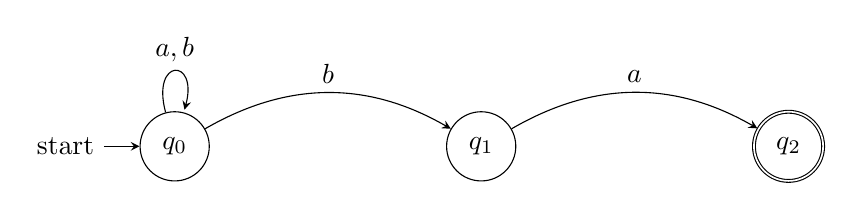
\begin{tikzpicture}[>=stealth,node distance=3cm,auto]
  % Stati
  \node[state,initial] (q0) {$q_0$};
  \node[state,right=of q0] (q1) {$q_1$};
  \node[state,accepting,right=of q1] (q2) {$q_2$};

  % Loop su q0
  \path[->]
    (q0) edge[loop above] node {$a,b$} (q0)
    % Transizione q0 --b--> q1
    (q0) edge[bend left] node {$b$} (q1)
    % Transizione q1 --a--> q2
    (q1) edge[bend left] node {$a$} (q2);
\end{tikzpicture}\\
\textit{Ora calcoliamo i nuovi stati grazie alla funzione di transizione  $\triangle$ del DFA:}\\
\begin{itemize}
    \item $A=\epsilon$-closure(0): \{0\}
    \item $\triangle(A,a)=\{\epsilon$-closure$(\underbrace{\text{mossa}(A,a)}_\text{esclusa partenza})\}=\epsilon$-closure$(\{0\})=\{0\}$
    \item $\triangle(A,b)=\epsilon$-closure$(\{0,1\})=\{0,1\} = B$
    \item $\triangle(B,a)=\epsilon$-closure$(\{0,2\})=\{0,2\}=C$
    \item $\triangle(B,b)=\epsilon$-closure$(\{0,1\})=\{0,1\}=B$
    \item $\triangle(C,a)=\epsilon$-closure$(\{0\})=\{0\}=A$
    \item $\triangle(C,b)\epsilon$-closure$(\{0,1\})=\{0,1\}=B$
\end{itemize}
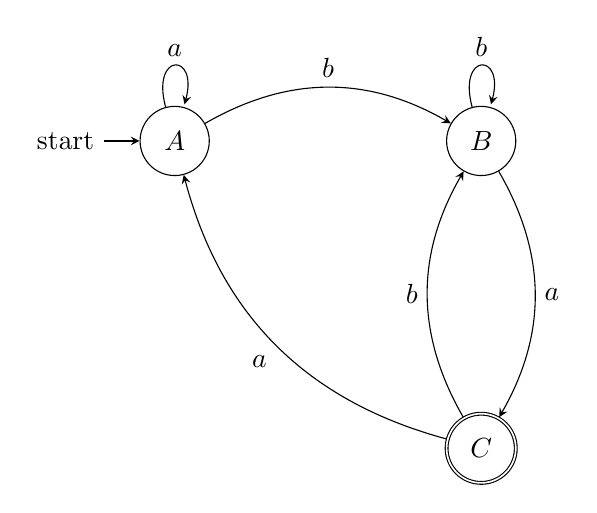
\begin{tikzpicture}[>=stealth,node distance=3cm,auto]

  % Stati
  \node[state,initial] (A) {$A$};
  \node[state,right=of A] (B) {$B$};
  \node[state,accepting,below=of B] (C) {$C$};

  % Transizioni
  \path[->]
    (A) edge[loop above] node {$a$} (A)
    (A) edge[bend left] node {$b$} (B)

    (B) edge[loop above] node {$b$} (B)
    (B) edge[bend left] node {$a$} (C)

    (C) edge[bend left] node {$a$} (A)
    (C) edge[bend left] node {$b$} (B);

\end{tikzpicture}\\
\textit{DFA ottenuto per costruzione per sottoinsiemi.\\
\vspace{1px}\\
La $\epsilon$-closure di $q$ e' l'insieme degli stati raggiungibile da $q$ solo con mosse $\epsilon$.\\
Se con un NFA ha cardinalita $n$ allora il suo DFA nel caso peggiore ha $2^n$ di cardinalita'.}
\end{mdframed}
\domanda{43}{Enunciare il teorema che dice che la classe dei linguaggi riconosciuti da NFA coincide con la classe dei linguaggi riconosciuti da DFA.}{Teorema: Sia $N=(\Sigma, Q, \delta, q_0, F)$ un NFA e sia $M_N$ l'automa ottenuto per sottoinsiemi. Allora $M_N$ e' un DFA e si ha che:
\begin{align}
    L[N]=L[M_N]
\end{align}}

\domanda{44}{Come si costruisce un NFA a partire da una espressione regolare, in modo tale che il linguaggio riconosciuto dall'NFA sia lo stesso del linguaggio associato all'espressione regolare?}{Dato $S=(a|b)^*ba$ \\
Partiamo dalla radice (bottom-up):}
\begin{mdframed}[backgroundcolor=grigiochiarissimo,
  linecolor=gray!50, linewidth=0.6pt,
  innertopmargin=6pt, innerbottommargin=12pt,
  innerleftmargin=8pt, innerrightmargin=8pt]
N[a]\\
  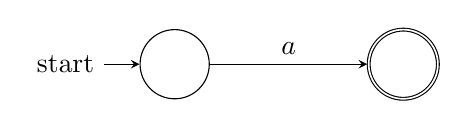
\begin{tikzpicture}[>=stealth,node distance=2cm,auto]
  \node[state,initial] (s0) {};
  \node[state,accepting,right=of s0] (s1) {};
  \path[->] (s0) edge node {$a$} (s1);
\end{tikzpicture}\\
N[b]\\
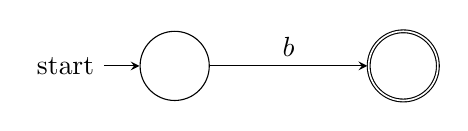
\begin{tikzpicture}[>=stealth,node distance=2cm,auto]
  \node[state,initial] (s0) {};
  \node[state,accepting,right=of s0] (s1) {};
  \path[->] (s0) edge node {$b$} (s1);
\end{tikzpicture}\\
N[a|b]\\
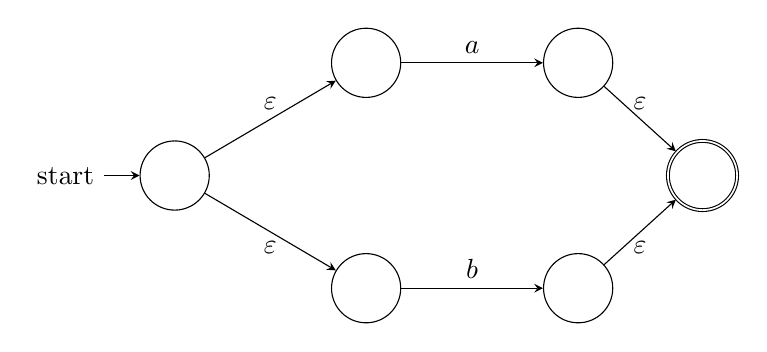
\begin{tikzpicture}[>=stealth,node distance=1.8cm,auto]

  % Stati
  \node[state,initial] (s0) {};
  \node[state,above right=0.8cm and 1.8cm of s0] (s1a) {};
  \node[state,below right=0.8cm and 1.8cm of s0] (s1b) {};
  \node[state,right=of s1a] (s2a) {};
  \node[state,right=of s1b] (s2b) {};
  \node[state,accepting,right=5.8cm of s0] (sf) {};

  % Transizioni
  \path[->]
    (s0) edge node[above] {$\varepsilon$} (s1a)
    (s0) edge node[below] {$\varepsilon$} (s1b)

    (s1a) edge node {$a$} (s2a)
    (s1b) edge node {$b$} (s2b)

    (s2a) edge node[above] {$\varepsilon$} (sf)
    (s2b) edge node[below] {$\varepsilon$} (sf);

\end{tikzpicture}\\
\begin{figure}[H]
  \centering
  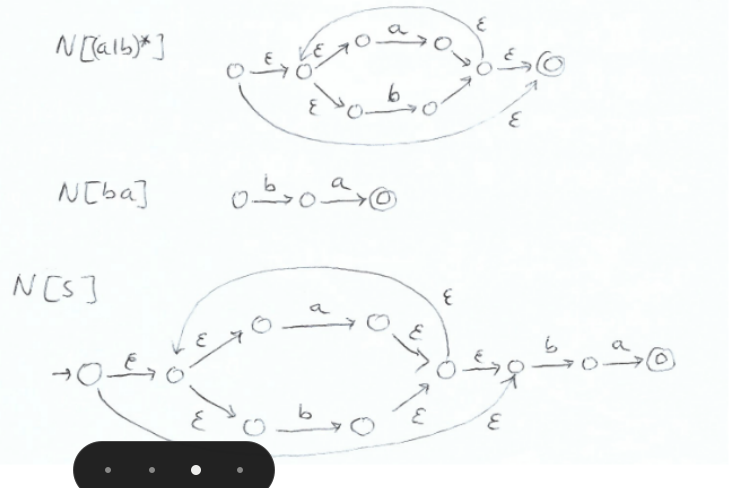
\includegraphics[height=10cm]{img/NFA.png}
\end{figure}



\end{mdframed}

\domanda{45}{Definizione di grammatica regolare.}{La dice grammatica $G$ e' regolare sse e' generata da un linguaggio regolare.\\
ESEMPIO:\\
\begin{align*}
    G := & \begin{cases}
        A \to aB \,|\, \epsilon \\
        B \to bA \,|\, \epsilon
    \end{cases}\\
    G := & A \to abA \,|\, a \,|\, \epsilon\\
    G := & (ab)^*(a|\epsilon)
\end{align*}}

\domanda{46}{Come si associa ad una grammatica regolare un equivalente NFA?}{
    \begin{center}
        NFA $\Rightarrow$ DFA $\Rightarrow$ Grammatica regolare
    \end{center}
}

\domanda{47}{Dato un DFA, come si costruisce una grammatica regolare equivalente?}{I nodi saranno i terminali, mentre gli archi i non terminali.}

\begin{mdframed}[backgroundcolor=grigiochiarissimo,
  linecolor=gray!50, linewidth=0.6pt,
  innertopmargin=6pt, innerbottommargin=12pt,
  innerleftmargin=8pt, innerrightmargin=8pt]
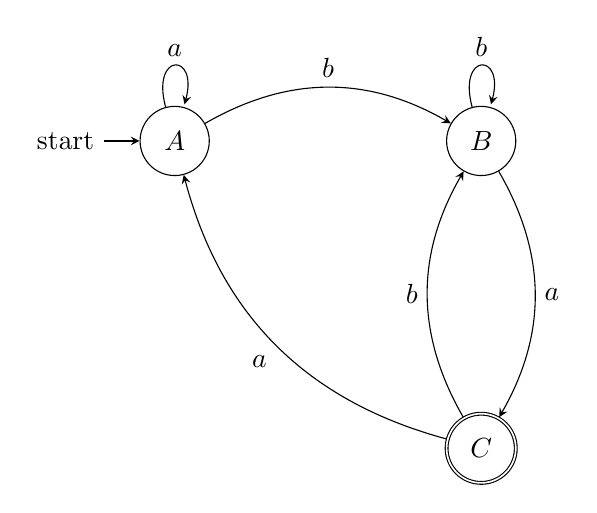
\begin{tikzpicture}[>=stealth,node distance=3cm,auto]

  % Stati
  \node[state,initial] (A) {$A$};
  \node[state,right=of A] (B) {$B$};
  \node[state,accepting,below=of B] (C) {$C$};

  % Transizioni
  \path[->]
    (A) edge[loop above] node {$a$} (A)
    (A) edge[bend left] node {$b$} (B)

    (B) edge[loop above] node {$b$} (B)
    (B) edge[bend left] node {$a$} (C)

    (C) edge[bend left] node {$a$} (A)
    (C) edge[bend left] node {$b$} (B);

\end{tikzpicture}\\
$     S \to A \\
     A \to aA \,|\, bB \\
     B \to aC \,|\, bB \\
     C \to aA \,|\, bB \,|\, \epsilon$
\end{mdframed}
\domanda{48}{Data una grammatica regolare, come si costruisce un'espressione regolare equivalente?}{Semplifichiamo la grammatica rimuovendo i simboli inutili\\
$ A \to aA \,|\, \epsilon \,|\, bc\\
C \to bC \,|\, \epsilon \,|\, aD \\
D \to aD \,|\, bD$ (questa non finisce mai)\\
diventa\\
$A \to aA \,|\, \epsilon \,|\, bC\\
C \to bC \,|\, \epsilon 
$\\
Ora ricaviamo l'espressione regolare associata:\\
$
C = b^*\\
A = a^*b^*$
}

\domanda{49}{Descrivere, con un diagramma riassuntivo, tutte le relazioni fra i formalismi introdotti: NFA, DFA, grammatiche regolari, espressioni regolari.}{
\begin{center}
\begin{tabular}{c c}
Grammatiche regolari $\Rightarrow$ NFA \\
$\Uparrow \hspace{4cm} \Downarrow$ \\
Espressioni regolari $\Leftarrow$ DFA \\
\end{tabular}
\end{center}
}

\domanda{50}{Definizione di stati equivalenti in un DFA. Quando due stati di un DFA sono distinguibili?}{Due stati sono equivalenti quando per ogni stringa $w \in \{\Sigma +\epsilon\}$:
\begin{align*}
  &\delta^*(q_0, w) \in F \iff \delta^*(q_1), w \in F\\
  & L[DFA, q_0] = L{DFA, q_1}
\end{align*}
Nota che $\delta^*$ e' la funzione di transizione completa su tutta la stringa.\\
\vspace{1px}\\
Due stati sono distinguibili quando:
\begin{align*}
  \delta^*(q,0, w) \in F \text{ e } \delta^*(q_1, w) \notin F
\end{align*}}

\domanda{51}{Come funziona l'algoritmo iterativo con tabella a scala per produrre le classi di equivalenza di stati di un DFA?}{Dato un DFA con $q_0, \dots, q_i$ stati e $q_i$ stato terminale, costruiamo la tabella a scala:
\begin{enumerate}
  \item Le $x$ sara' numerato da $0$ a $i-1$
  \item Le $y$ sara' numerato da $i$ a $1$
  \item Flag su l'incrocio fra tutti gli elementi con gli stati terminali
  \item Controlliamo per ogni cella , ip. $q_k$ $q_m$, ogni movimento per ogni lettera, se otteniamo anche solo una nuova coppia che e' flaggata allora flaggiamo anche qua
  \item Se abbiamo delle coppie di stati non flaggate allora sono equivalenti
  \item Costruiamo un nuovo grafo unendo le coppie equivalenti
  \item Ricontroliamo
\end{enumerate}}

\domanda{52}{Una volta determinate le classi di equivalenza degli stati di un DFA, come si costruisce l'automa minimo associato?}{
  \begin{enumerate}
    \item Date le coppie di stati di equivalenza
    \item Costriamo un nuovo grafo unendo le coppie identica fra le loro relazioni
    \item Ricostruiamo un nuovo DFA
    \item Controlliamo se questo sia minimo
  \end{enumerate}
Ora abbiamo un DFA minimo!
}

\domanda{53}{Cos'e Lex? Qual e il suo input e il suo output?}{Lex e' un generatore di Lexer:
\begin{itemize}
  \item Input: file \texttt{.l} nel quale specifichiamo le definizioni regolare
  \item Output: file \texttt{.c} che realizza l'automa riconoscitore
\end{itemize}}

\domanda{54}{Qual e la struttura di un file .l? Come funziona l'analizzatore lessicale prodotto da Lex?}{E' diviso in 3 parti:
\begin{enumerate}
  \item Dichiarazioni (definizioni regolari)
  \item Regole (pattern $\Rightarrow$ C code)
  \item Funzioni ausiliarie
\end{enumerate}
L'automa in C implementa il DFA riconoscitore delle espressioni regolari e restituisce <TOKEN, lessemma>.}

\domanda{55}{Come si interfaccia Lex con Yacc?}{Yacc chiama Lex attraverso una funzione \texttt{yylex()}, lex ritorna la tuple <TOKEN, lessemma> e YACC e' un generatore di parser (analizzatore sintattico).}

\domanda{56}{Intestazione e dimostrazione del pumping lemma.}{Se $L$ e' un linguaggio regolare allora $\exists N\geq 1$ t.c. per ogni stringa accettata in $L$ ($uvw \in L$) e' $|uvw|\geq N$: 
\begin{itemize}
  \item $|uv| \leq N$
  \item $v \geq 1$
  \item $\forall k \geq 0 \quad uv^kw \in L$
\end{itemize}
\texttt{DIMOSTRAZIONE}: Sia $DFA=(\Sigma, Q, \delta, q_0, F)$ che genera $L$:
\begin{align}
  & |DFA| = N
\end{align}
Consideriamo una stringa $|uvw|\geq N$, durante la lettura delle prime $N$ lettere siamo passati da $N+1$ stati (anche iniziale), ed essendo un DFA per definione abbiamo solo $N$ stati. Quindi in uno stato ci siamo passati piu' volte.\\
Chiamiamo $q_i$ lo stato passato piu' volte, definiamo che
\begin{itemize}
  \item $x$ e' la parte di string fino a $q_i$
  \item $v$ e' la parte di loop 
  \item $w$ e' la parte post $q_i$
\end{itemize}
Ovvero che allo stato $q_i$ se leggiamo certi caratteri (quelli dentro $v$) otteniamo 
\begin{align*}
  \delta^*(q_i, v) = q_i
\end{align*}
la lunghezza di $v$ non importa tanto e' un loop che consuma tutti i caratteri compatibili con il loop, ovvero
\begin{align*}
  uv^kw \in L \quad \forall k \geq 0
\end{align*}}

\domanda{57}{Come si puo utilizzare il pumping lemma (a rovescio) per dimostrare che un linguaggio non e regolare?}{ 
Dimostriamo che $L=\{a^nb^n | n \geq 1\}$ non sia regolare.\\
\vspace{1px}\\
Assumiamo per assurdo che $L$ sia regolare, allora vale il pumping lemma che ci dice:
\begin{itemize}
  \item Fissata una lunghezza $N \geq 1$
  \item Data la stringa $uvw \in L$ e $|uvw| \geq N$: \begin{enumerate}
    \item $|uv| \leq N$
    \item $|v| \geq 1$
    \item $\forall k \geq 0 \quad uv^kw \in L$
  \end{enumerate}
  La nostra stringa e' $a^Nb^N$, quindi $uv=a^N$ e $w=b^N$.\\
  Scomponiamo $uv=a^N$ in $u=a^m$ e $v=a^{N-m}$ ($m<N$), pero' per n.3 sappiamo che 
  \begin{align*}
    & uv^kw \in L\\
    \Rightarrow & a^m a^{k(N-m)}b^N \in L \quad \forall m<N \quad \forall k \geq 0 \\
    \Rightarrow & a^m a^{kN-km} b^N
  \end{align*}
  Ipotizziamo $N=2$, $k=2$:
  \begin{align*}
    \Rightarrow & a^m a^{4-2m} b^2
  \end{align*}
  Ipotizziamo $m=1$
  \begin{align*}
    \Rightarrow & a^1 a^2 b^2 \\
    \Rightarrow & aaabb \notin L
  \end{align*}
  $\to$ assurdo! Quindi $L$ non e' regolare.\\
\end{itemize}}

\domanda{58}{Quali sono le proprieta di chiusura dei linguaggi regolari? Quali proprieta si possono decidere (ovvero verificare algoritmicamente)?}{La classe regolare e' chiusa per tutto, ovvero unione, intersezione, concatenazione, Kleene, complemento.}

% ----------------------------------------------------------------
\subsection{Capitolo 4 -- Analisi sintattica, linguaggi liberi}
% ----------------------------------------------------------------

\domanda{59}{Cosa si intende per analisi sintattica? Cos'e un parser?}{L'analisi sintattica e' la fase del compilatore dove data una lista di token si controlla che rispetti la grammatica del linguaggio (ordine dei token). Il parser e' il componente che esegue l'analisi sintattica e restituisce AST.}

\domanda{60}{Definizione di automa a pila nondeterministico (PDA). Definizione di configurazione (o descrizione istantanea), mossa in un passo e mossa in piu passi.}{Un PDA (automa a pila non-deterministico) e' una 7-pla $(\Sigma, Q, \Gamma, \delta, q_0, \bot, F)$ dove:
\begin{itemize}
  \item $\Sigma$: input
  \item $Q$: stati totali
  \item $\Gamma$: insieme simboli pila
  \item $\delta$: funzione di transizione
  \item $q_0$: stato iniziale
  \item $\bot \in \Gamma$: simbolo iniziale sulla pila
  \item $F$: stato finale
\end{itemize}}

\domanda{61}{Definizione di linguaggio accettato da un PDA per stato finale o per pila vuota. Sono equivalenti queste due modalita di riconoscimento?}{Due modalita' di riconoscimento:
\begin{itemize}
  \item Stato finale:
  \begin{align*}
    \{w \in \Sigma^* | (q_0, w, \bot) \vdash^*_N (q_f, \epsilon, \gamma ) \quad q_f \in F\}
  \end{align*}
  \item Pila vuota:
   \begin{align*}
    \{w \in \Sigma^* | (q_0, w, \bot)\vdash^*_N (q_f, \epsilon, \epsilon) \quad q_f \in F\} 
  \end{align*}
\end{itemize}
\begin{itemize}
  \item $q_0$ stato iniziale
  \item $w$ stringa ancora non letta
  \item $\bot$ pila vuota
  \item $q_f$ stato finale
  \item $\epsilon$ lettera terminale
  \item $\gamma$ contenuto pila (completa)
\end{itemize}
Le due modalita' sono equivalenti per un teorema.}

\domanda{62}{Mostrare come data una grammatica libera G sia possibile costruire un PDA P equivalente. E possibile costruire, dato un PDA P, una grammatica equivalente G? Concludere che la classe dei linguaggi liberi coincide con la classe dei linguaggi riconosciuti da PDA.}{Data la grammatica libera $G$:\\
$G=
\begin{cases}
  A \to aAb \mid \epsilon
\end{cases}$
}
\begin{mdframed}[backgroundcolor=grigiochiarissimo,
  linecolor=gray!50, linewidth=0.6pt,
  innertopmargin=6pt, innerbottommargin=12pt,
  innerleftmargin=8pt, innerrightmargin=8pt]
\textit{PDA stato finale:}\\
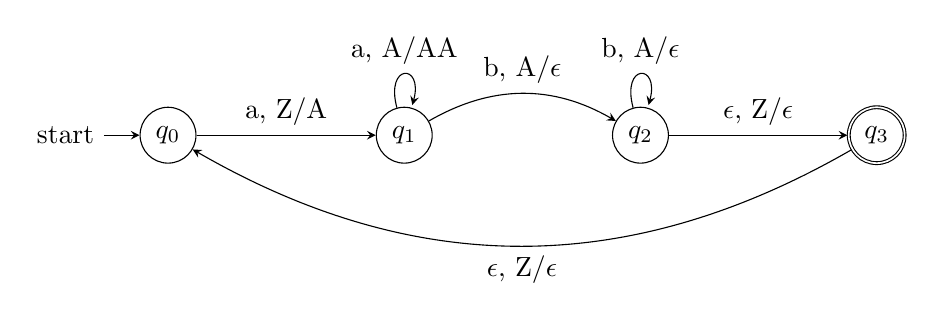
\begin{tikzpicture}[>=stealth,node distance=3cm,auto]
  \tikzstyle{state}=[circle,draw,minimum size=18pt]

  \node[state,initial] (q0) {$q_0$};
  \node[state] (q1) [right of=q0] {$q_1$};
  \node[state] (q2) [right of=q1] {$q_2$};
  \node[state,accepting] (q3) [right of=q2] {$q_3$};

  \path[->]
    (q0) edge node {a, Z/A} (q1)
    (q1) edge[loop above] node {a, A/AA} ()
    (q1) edge[bend left] node {b, A/$\epsilon$} (q2)
    (q2) edge[loop above] node {b, A/$\epsilon$} ()
    (q2) edge node {$\epsilon$, Z/$\epsilon$} (q3)    
    (q3) edge[bend left] node {$\epsilon$, Z/$\epsilon$} (q0);
\end{tikzpicture}\\
\vspace{1px}\\
Si, dato il PDA qua sopra sappiamo che:
\begin{itemize}
  \item Inizia con $(a \mid \epsilon)$
  \item Contiene $a^*$
  \item Contiene $b^*$
\end{itemize}
Quindi $L[PDA]=a^*b^*$, che si puo' scrivere come: $S \to aSb \mid \epsilon$.\\
\vspace{1px}\\
Quindi abbiamo mostrato come dalla grammatica $G$ abbiamo ottenuto un PDA che a sua volta ha generato una grammatica, tutte queste coincidono nello stesso linguaggio.
\end{mdframed}
\domanda{63}{Quali sono le proprieta di chiusura dei linguaggi liberi? L'intersezione di un linguaggio libero con un regolare e un linguaggio libero?}{I linguaggi liberi sono chiusi per:
\begin{itemize}
  \item Unione
  \item Concatenazione
  \item Kleene
\end{itemize}
Mentre se l'intersezione tra un libero e un regolare e' sempre libero (chiuso).}

\domanda{64}{Intestazione e dimostrazione del Pumping Theorem per i linguaggi liberi.}{Fissiamo $N \geq 1$, allora $uvwxy \in L$ e $|uvwxy||\geq N:$\\
\begin{itemize}
  \item $|vwx| \leq N$ 
  \item $|vx| \geq 1$
  \item $\forall k \geq 0 \quad uv^kwx^ky \in L$
\end{itemize}}

\domanda{65}{Come si puo utilizzare tale teorema (a rovescio) per dimostrare che un linguaggio non e libero?}{Ipotizziamo per assurdo che $L$ sia libero, allora $\forall N \geq 1$ e $\forall uvwxy \in L$ t.c. $|uvwxy| \geq N$. Allora vale per pumping theorem libero:
\begin{itemize}
  \item $|vwx| \leq N$ 
  \item $|vx| \geq 1$
  \item $\forall k \geq 0 \quad uv^kwx^ky \in L$
\end{itemize}
Fissiamo un valore $k$ t.c. $uv^kwx^ky \notin L$\\
$\Rightarrow$ $L$ non e' libero!}

\domanda{66}{Classificazione di Chomsky delle grammatiche e dei linguaggi. Definizione di grammatica dipendente dal contesto e di grammatica monotona. Quale tipo di automi corrisponde ad ogni classe?}{
  \begin{enumerate}
    \item Grammatiche regolari (DFA-NFA)
    \item Grammatiche libere da contesto (PDA)
    \item Grammatiche dipendeti da contesto (LBA):
    \begin{align*}
      aA \to B \quad \text{ Nota come dipende da 2 argomenti a sinistra!}
    \end{align*}
    \item \begin{itemize}
      \item Grammatiche Monotone: non acconsente di accorciare ($aA \to B$)
    \begin{align*}
        A \to B \quad \text{ con } |A| \leq |B|
    \end{align*}
    \item Grammatiche generali (Macchine di Turing)
    \end{itemize}
  \end{enumerate}
}

\domanda{67}{Definizione di DPDA (automa a pila deterministico) e di linguaggio libero deterministico.}{Un linguaggio e' libero deterministico se e' accettato per stato finale da un DPDA:
\begin{align*}
  \forall q \in Q \quad \forall z \in \Gamma \quad \forall a \in \Sigma^* \quad \mid \delta(q,a,z)\mid \leq 1
\end{align*}
Ovvero ad ogni stato se dobbiamo mettere $a$ dentro la pila possiamo prendere 1 sola strada possibile.}

\domanda{68}{La classe dei linguaggi liberi deterministici e strettamente inclusa in quella dei linguaggi liberi? Contiene strettamente la classe dei linguaggi regolari?}{
  \begin{align*}
    & REG \subset DCFG \subset CFG \\
    & NFA/DFA \subset DPDA \subset PDA
  \end{align*}
}

\domanda{69}{Che cosa dice la prefix property e perche e interessante per i DPDA?}{Un linguaggio libero deterministico gode della prefix property quando nessuna parola e' prefisso di un'altra. \\
Tipo $L=\{a, ab\}$ il DPDA dopo aver letto $a$ non saprebbe se chiudere o continuare. Quindi non sarebbe deterministico.}

\domanda{70}{Usando un endmarker \$, si puo riconoscere un linguaggio libero deterministico che non gode della prefix property anche per pila vuota? Come?}{Esattamente $\$$ serve proprio per far riconoscere per pila vuota un DPDA che non gode di prefix property.\\
Inseriamo il simbolo $\$$ al fine del linguaggio:
\begin{align*}
  L \to L\$
\end{align*}
Cosi quando leggiamo $\$$ siamo sicuri che sia finito.}

\domanda{71}{Un linguaggio libero deterministico e ambiguo?}{Non sempre dipende, un DPDA e' deterministico ma possono esistere gramamtiche ambigue che generano il linguaggio.}

\domanda{72}{Proprieta di chiusura dei linguaggi liberi deterministici: chiusi per complementazione, ma non per intersezione ne per unione.}{
  \begin{itemize}
    \item Complemento
    \item Intersezione con i regolari
  \end{itemize}
}

\domanda{73}{Da cosa si parte per costruire un analizzatore sintattico (ovvero parser)? Da una espressione regolare? Da una grammatica libera? Da un PDA?}{Si utilizza una CFG. Il PDA lo utilizziamo sono come modello per il riconoscimento.\\
L'espressione regolare non va bene perche' e' limitante esprimento un linguaggio regolare (NFA/DFA).}

\domanda{74}{Cosa prende in input e cosa produce in output un parser?}{Prende in input una tuple <TOKEN, lessemma> e restituisce in output un AST.}

\domanda{75}{Che differenza c'e tra un parser nondeterministico ed uno deterministico?}{Il parser determinstico e' quello "classico" che prende scelte assolute, mentre quello nondeterministico utilizza il backtracking quando una scelta e' errata.}

\domanda{76}{Quali sono le due tecniche essenziali per costruire parsers?}{Le due tecniche sono:
\begin{itemize}
  \item Top-down: data la stringa in input $w$ partiamo dal simbolo iniziale $S$
  \item Bottom-up: data la stringa in input $w$ cerchiamo di ridurre fino a $S$
\end{itemize}}

\domanda{77}{Le tecniche top-down e bottom-up in che cosa differiscono?}{
  \begin{itemize}
    \item Top-down: partiamo con $S$ sulla pila e la espandiamo a seconda dell'input
    \item Bottom-up: partendo dalla pila vuota pushiamo (shift) gli input sulla pila, quando poi abbiamo una combinazione li traduciamo in Terminali (reduce) e continiamo fino ad avere stato iniziale $S$
  \end{itemize}
}

\domanda{78}{Quali tipi di grammatiche non sono adatte al top-down parsing? Quali tipi di produzioni sono poco adatte al bottom-up parsing?}{
Il Top-down non supporta il \texttt{left recursion}
\begin{align*}
  A \to Aa \mid b
\end{align*}
Il Bottom-up ha problemi per i \texttt{conflitti shift/reduce}:
\begin{align*}
  E \to E+E \mid id
\end{align*}
Top-down e Bottom-up DETERMINISTICI non supportano le $\epsilon$-produzioni:
\begin{align*}
  A \to \epsilon
\end{align*}
}

\domanda{79}{Cosa sono le produzioni epsilon e cosa sono i simboli non-terminali annullabili?}{Le $\epsilon$-produzioni sono la riduzione da 
\begin{align*}
  & A \to \epsilon \\
  & L(G) = L(G) \backslash \{\epsilon\}
\end{align*}
non sono compatibili con i DPDA.\\
\vspace{1px}\\
I simboli non-terminali annullabili sono quelli che si riducono a $\epsilon$-produzioni (anche indirettamente).
}

\domanda{80}{Come si puo trasformare una grammatica G che contiene produzioni epsilon in una grammatica G' che non ne contiene, preservando il linguaggio a meno di epsilon?}{Se $\epsilon \in L(G)$ e vogliamo $L(G')=L(G)\backslash \{\epsilon\}$ allora:
\begin{itemize}
  \item Eliminiamo i non-terminali annullabili
  \item Mettiamo un nuovo simbolo iniziale $S' \to S \mid \epsilon$
\end{itemize}}

\domanda{81}{Cosa sono le produzioni unitarie e cosa sono le coppie unitarie?}{Dati i non-terminali $A,B$ li definiamo unitari se
\begin{align*}
  A \to B
\end{align*}
Li definiamo coppie unitarie se
\begin{align*}
  A \to^* B \text{ attraverso solo coppie unitarie}
\end{align*}}

\domanda{82}{Come si puo trasformare una grammatica G che contiene produzioni unitarie in una equivalente G' che non ne contiene?}{Possiamo sostituire tutte le produzioni unitarie $A\to B$ direttamente con le produzioni di $B$.}

\domanda{83}{Data una grammatica G, quali sono i suoi simboli utili? Quali sono i suoi simboli generatori? Quali i suoi simboli raggiungibili?}{Un non-terminale e' generatore quando riesce a derivare almeno una stringa di soli terminali
\begin{align*}
  A \to^* w \quad w \in \Sigma^*
\end{align*}
Un simbolo (terminale e non) e' raggiungibile quando si puo' produrre partendo da $S$.\\
Un simbolo e' utilie quando e' generatore e raggiungibile.}

\domanda{84}{Come si calcolano i generatori? Come si calcolano i raggiungibili?}{I generatori si calcolano:
\begin{itemize}
  \item Segniamo tutti i non-terminali che si riducono con 1 step a terminale (stringhe)
  \item Segniamo ora tutti i non-terminali che si riducono a i non-terminale di prima
  \item Cosi via
  \item I restanti alla fine sono i non generatori.
\end{itemize}
I simboli non raggiungibili si calcolano:
\begin{itemize}
  \item Iteriamo da $S$ ogni possibile strada presa dalle riduzioni
  \item Quando arriviamo a un terminale (stringhe) lo flaggiamo
  \item Backtracking alla divarazione precedente
  \item Ripetiamo finche non abbiamo passato tutte le divariazioni
  \item I non flaggati sono non raggiungibili
\end{itemize}}

\domanda{85}{In che modo si eliminano i simboli inutili di una grammatica? E importante l'ordine delle operazioni da svolgere?}{Calcoliamo i simboli non-terminali generatori, quelli non-generatori li cancelliamo ovonque. \\
Calcoliamo i simboli raggiungibili, i restanti li cancelliamo. Ora abbiamo solo simboli utili.}

\domanda{86}{Quando si dice che una grammatica e ricorsiva sinistra? Come si elimina la ricorsione sinistra immediata? E quella non immediata? Perche serve eliminare la ricorsione sinistra?}{Una grammatica e' ricorsiva sinistra (left recursion) quando abbiamo
\begin{align*}
  A \to Aa
\end{align*}
Ovvero il primo carattere della riduzione e' il non-terminale stesso che si e' appena ridotto.\\
Per rimuoverla se abbiamo:
\begin{align*}
  A \to Aa | B \mid 
\end{align*}
Definiamo un nuovo non-terminale per produrre ricorsivamente a destra "$a$" chiamato $A'$
\begin{align*}
  A' \to aA' \mid \epsilon
\end{align*}
e modifichiamo $A$ in modo che prima chiamiamo $B$ e poi generiamo gli "$a$":
\begin{align*}
  &A \to BA' \\
  &A' \to aA' \mid \epsilon
\end{align*}}

\domanda{87}{Cosa vuol dire fattorizzare a sinistra una grammatica? Perche serve fattorizzare?}{In un DPDA se abbiamo
\begin{align*}
  A \to aB \mid a
\end{align*}
non sappiamo cosa scegliere. Quindi creiamo un nuovo terminale $A'$ che ci genera la parte non-comune:
\begin{align*}
  &A \to aA'\\
  &A' \to B
\end{align*}
Questo ci permette di avere lo stesso linguaggio ma con una grammatica che vada su un parser deterministico.}

\domanda{88}{Cos'e un parser a discesa ricorsiva?}{Un parser a discesa ricorsiva e' un parser top-down che ricostruisce partendo da $S$ attraverso dichiarazioni ricorsive.\\
Per il linguaggio
\begin{align*}
  &E \to T + E \mid T \\
  &T \to id
\end{align*}
lo definiamo con:
\[
\begin{aligned}
E(): \quad & T() \\
          & \text{if } next == '+' \text{ then} \\
          & \quad match('+') \\
          & \quad E() \\[2mm]
T(): \quad & match(id)
\end{aligned}
\]
}

\domanda{89}{Definizione di First(a) e di Follow(A).}{First e' l'insieme dei terminali che sono in prima posizione dal terminale $A$:
\begin{align*}
  &A \to aA \mid epsilon\\
  &First(A)=\{a, \epsilon\}
\end{align*}
Follow del non-terminale $X$ e' l'insieme dei terminali che spuntano dopo per definizione o riduzione ad $X$:
\begin{align*}
  &S \to Ab \mid c \\
  &A \to aA \mid \epsilon\\
  &Follow(S) = \{\$\}\\
  &Follow(A)=\{b\}
\end{align*}}

\domanda{90}{Algoritmi per calcolare First(a) e Follow(A).}{
First:
\begin{itemize}
  \item Per ogni terminale $x$ facciamo che $First(x)=\{x\}$
  \item Per ogni non-terminale $A$:
  \begin{itemize}
    \item Per ogni sua produzione $x$:
    \begin{itemize}
      \item Per ogni carattere di $x$ chiamato $c$:
      \begin{itemize}
      \item $First(A)+=First(c)$
    \end{itemize}
    \end{itemize}
  \end{itemize}
\end{itemize}
Follow:
\begin{itemize}
  \item $Follow(S)=\{\$\}$
  \item Per ogni non-terminale $A$:
  \begin{itemize}
    \item Per ogni sua produzione $x$:
    \begin{itemize}
      \item Per ogni carattere di $x$ chiamato $c$:
      \begin{itemize}
        \item if $A == S$ and $c$ is ultimo in $x$: $Follow(A)+=\{\epsilon\}$
        \item else if $c$ is not ultimo in $x$: $Follow(c)+=First(c+1)\backslash \{\epsilon\}$
      \end{itemize}
    \end{itemize}
  \end{itemize}
\end{itemize}
}

\domanda{91}{Come e fatta e come si riempie una tabella di parsing LL(1)?}{Righe non-terminali, Colonne terminali.\\
Dalle produzioni per ogni per ogni $c \in First(A)$ compiliamo la cella $(A, x)$ con la produzione $A \to x\dots$. \\
Mentre i $c \in Follow(A)$ ci servono per ridurre $A \to \epsilon$ quando leggiamo $c$.}

\domanda{92}{Quando una grammatica G si dice di classe LL(1)? Quali sono le condizioni necessarie e sufficienti per G affinche sia di classe LL(1)?}{Una grammatica $G$ e' LL(1) se la sua tabella di parsing LL(1) contiene al max. 1 produzione per ogni casella.\\
E' LL(1) quando per ogni 
\begin{align*}
  A \to B \mid C
\end{align*}
abbiamo
\begin{enumerate}
  \item $First(B)\cap First(C) = \emptyset$
  \item Se $\epsilon \in Follow(B)$ allora $Follow(A) \cap Fist(C) = \emptyset$
  \item Se $\epsilon \in Follow(C)$ allora $Follow(A) \cap Fist(B) = \emptyset$
\end{enumerate}
Nota che 2/3 servono perche se avessimo caratteri in comuni non sapremmo se ridurre $A \to C \to \epsilon + B \to c$ oppure $A \to B \to c$}

\domanda{93}{Perche un parser di questo tipo e chiamato LL?}{
  \begin{center}
    Left-to-right $\qquad$ Leftmost
  \end{center}
  Perche' e' un parser top-down che partendo da $S$ consuma da sinistra a destra gli input per arrivare allo stato finale.
}

\domanda{94}{Come funziona il parser LL(1) con una pila?}{A seconda di quello che e' il carattere in lettura pushiamo nello stack la produzione della sua cella in base al non terminale dello stack per poi consumarlo da entrambi i lati. Continiamo finche' non abbiamo piu' caratteri in input e la pila con il terminatore.}

\domanda{95}{E vero che ogni linguaggio regolare e pure LL(1)?}{Si perche ogni grammatica regolare puo' essere trasformata in una LL(1) compatibile, dato che le sue restrizioni forti permettono di non avere mai conflitti in LL(1).}

\domanda{96}{Come sono definiti First$_k$(a) e Follow$_k$(A) per $k \geq 2$?}{
Le definizioni di FIRST$_k$ e FOLLOW$_k$ estendono FIRST e FOLLOW considerando stringhe terminali di lunghezza al più $k$.\\
\textbf{FIRST$_k$:}
Per una stringa $\alpha$, FIRST$_k(\alpha)$ è l’insieme delle stringhe terminali $w$ tali che:
\[
\alpha \Rightarrow^* w\beta \quad \text{con } |w| \le k
\]
cioè tutte le possibili stringhe di terminali (lunghezza $\leq$ $k$) che possono apparire come prefisso di una derivazione di $\alpha$.\\
\vspace{2mm}\\
\textbf{FOLLOW$_k$:}
Per un non-terminale $A$, FOLLOW$_k(A)$ è l’insieme delle stringhe terminali $w$ tali che:
\[
S \Rightarrow^* \alpha A w \beta \quad \text{con } |w| \le k
\]
cioè tutte le stringhe di terminali (lunghezza $\leq$ $k$) che possono comparire immediatamente a destra di $A$ in una derivazione.
}

\domanda{97}{Come si definisce una grammatica LL(k)? Ed un linguaggio LL(k)? Come si relazionano tra di loro?}{LL(k) e' una quadrupla $(NT, T, \delta, S)$ con:
\begin{itemize}
  \item $NT$ insieme non terminali
  \item $T$ insieme terminali
  \item $\delta$ funzione transazione
  \item $S$ simbolo iniziale
\end{itemize}
Un linguaggio $L \subseteq \Sigma^*$ e' LL(k) se esiste almeno una grammatica $LL(k)$ che lo genera.}

\domanda{98}{Che relazione esiste tra grammatiche LL(k) e grammatiche ambigue? E con le grammatiche ricorsive sinistre?}{Una grammatica LL(k) non e':
\begin{itemize}
  \item ambigua
  \item ricorsiva sinistra
\end{itemize}
Ogni grammatica LL(k) non e' ambigua e ogni grammatica ambigua e' non LL(k).}

\domanda{99}{Esistono linguaggi liberi che non sono LL(k) per nessun k? Ed esistono linguaggi liberi deterministici che non sono LL(k) per nessun k?}{Si perche' abbiamo che
\begin{align*}
  LL(k) \subset DCFG \subset CFG
\end{align*}
Quindi essendo una relazione stretta alcuni linguaggi non esistono nel sottoinsieme minore.}

\domanda{100}{Cos'e un parser bottom-up (o shift-reduce)? Qual e il suo input e il suo output? Perche sono chiamati parser LR?}{Un parser bottom-up parte dalla pila vuota e attraverso gli shift-reduce arriviamo allo stato iniziale $S$.\\
Il suo input sono una lista di token, e il suo output e' un ast.\\
Si chiama LR perche' e left-to-right rightmost, ovvero legge da sinistra a destra ma partiamo dalla pila vuota.}

\domanda{101}{Che tipo di conflitti si possono presentare in un parser del genere? Quando si presenta un conflitto (shift/reduce o reduce/reduce), quale azione bisogna scegliere?}{Possiamo avere conflitto shift-reduce o reduce-reduce ovvero momenti che il parser dove scegliere non deterministicamente una strada.\\
Se la grammatica e' LR(k) allora il problema shift-reduce o reduce-reduce non si pone.}
\domanda{102}{Cos'e un prefisso viabile? Come lo si definisce in termini di una grammatica?}{
Le stringhe che otteniamo durante il parsing bottom-up corretto si chiamano
prefissi viabili.\\
Data la grammatica $G = (NT, T, \delta, S)$, definiamo prefisso viabile:
\[
\{\, a \in (NT \cup T)^*
\mid
\exists\, \beta, A, w, \gamma :
S \Rightarrow^* \beta A w \Rightarrow \beta\gamma w
\ \land\
a \preceq \beta\gamma
\,\}.
\]
}


\domanda{103}{Cos'e un item LR(0)? Come si generano tutti gli item di una grammatica (aumentata con un simbolo iniziale nuovo S')?}{Gli item in $LR(0)$ indicano quali prefissi viabile abbiamo riconociuto e quale simbolo ci stiamo aspettando.\\
\vspace{1px}\\
Dato $S\to A_1\dots A_n$\\
Generiamo un item per ogni posizione:
\begin{itemize}
  \item $S' \to . S$
  \item $S' \to S .$
  \item $S \to . A_1\dots A_n$
  \item $S \to A_1 . \dots A_n$
  \item $\vdots$
  \item $S \to A_1\dots A_n .$
  \item $A \to . a$
  \item $A \to . a$
\end{itemize}
Se abbiamo $S \to \epsilon$ mettiamo $S \to .$.\\
Nota come se abbiamo dopo un punto un terminale espandiamo anche lui.}

\domanda{104}{Come e fatto il NFA dei prefissi viabili? Come si ricava il DFA dei prefissi viabili, detto anche automa canonico LR(0)?}{Data la grammatica estesa $G$:
\begin{itemize}
  \item $q_0 = [S' \to .S]$
  \item $q_i$ = \begin{itemize}
    \item Se abbiamo un NT mettiamo una transizione a costo $\epsilon$ tipo $[A \to B.a]$
    \item Se abbiamo un T mettiamo una transizione a costo $a$ tipo $[A \to a.B]$
  \end{itemize}
\end{itemize}
Quindi per ogni transizione in $G$ abbiamo uno stato nel NFA.\\
\vspace{1px}\\
Il DFA (automa canonico LR(0)) lo otteniamo:
\begin{enumerate}
  \item Costruzione per sottoinsiemi
  \item Clos(x) e Goto(I, x)
\end{enumerate}}

\domanda{105}{Come e fatta una tabella di parsing LR(0)? Come la si riempie a partire dall'automa canonico LR(0)? Quando una grammatica e di classe LR(0)?}{Dato DFA automa canonico LR(0) facciamo una tabella
\begin{itemize}
  \item righe: $1$ fino a $|DFA|$
  \item colonne: $T \cup NT \cup \{\$\}$
\end{itemize}
Se dallo stato $q_i$ abbiamo un T che vada a $k$ allora nella casella $(i, T)$ mettiamo $goto(k)$.\\
Se dallo stato $q_i$ abbiamo un NT che vada a $k$ allora nella casella $(i, NT)$ mettiamo $shift(k)$.\\
\vspace{1px}\\
Una grammatica e' LR(0) quando la sua tabella di parsing LR(0) non ha conflitti.}

\domanda{106}{Come e fatto il parser LR(0) che utilizza la tabella di parsing LR(0)? Quanti stack servono?}{\begin{itemize}
  \item Automa che genera tabella LR(0) 
  \item 1 Stack che indica il percorso degli stati (tipo [0,2,3])
  \item Tabella compilata LR(0)
  \item Input
\end{itemize}}

\domanda{107}{Esistono grammatiche non LR(0)? Fare un esempio semplice.}{Si non avendo lookhaed non riesci a risolvere:
\begin{align*}
  S \to aS \mid a
\end{align*}
oppure con ricorsione sinistra:
\begin{align*}
  S \to Sa \mid a
\end{align*}
Non sappiamo se leggiamo "a" se derivi da $Sa$ o $a$.\\
Questo perche' $First(S)\cap Follow(S) \neq \emptyset.$}

\domanda{108}{Come e fatta e come si riempie una tabella di parsing SLR(1)? Cosa vuol dire l'acronimo SLR? Perche si mette 1 come parametro?}{Attraverso 1 parametro di $lookhaed$ riusciamo ad ampliare il linguaggio di LR(0) riducendo i conflitti shift-reduce. Infatti
\begin{align*}
  LR(0) \subset SRL(1)
\end{align*}
Partendo da automa DFA LR(0) riusciamo a modificarlo attraverso 1 simbolo di lookhaed rispettivamente $Follow_1$.\\
SLR significa: "simple left-to-right rightmost", diciamo \texttt{simple} perche rispetto LR(1) la tecnica di seguire i $Follow$ e' banale e meno precisa.\\
Per definizione ci serve almeno 1 parametro, infatti SLR(0) non esiste.}

\domanda{109}{Quando una grammatica e di classe SLR(1)? Esistono grammatiche non di classe SLR(1)?}{Definiamo $G=(NT, T, \delta, S)$ grammatica SLR(1) se la sua tabella di parsing LR(0) + 1 simbolo di lookhaed basata sui i $Follow$ non contiene conflitti.\\
Si, esistono grammatiche non SLR(1) anche qua possiamo avere conflitti shift-reduce.}

\domanda{110}{Cos'e un item LR(1)? Come si costruisce il NFA LR(1)? E come l'automa canonico LR(1)?}{Un item LR(0) e' tipo:
\begin{align*}
  A \to a.
\end{align*}
mentre un item LR(1) e'
\begin{align*}
  A \to a. \, , a
\end{align*}
Ovvero possiamo produrre $A \to a$ solo se il prossimo simbolo e' un "a".\\
\vspace{1px}\\
NFA LR(1):
\begin{itemize}
  \item $q_0 = [S' \to .S , \mathdollar]$ 
  \item $q_i$ = \begin{itemize}
    \item Da $[A \to \omega . xB, a]$ abbiamo una transizione di costo $x \in T$ per andare allo stato $[A \to \omega x . B, a]$
    \item Da $[A \to \omega . xB, a]$ abbiamo una transizione di costo $\epsilon$ per andare allo stato $[A \to \omega x.B, a]$ per ogni produzione di $x$
  \end{itemize}
\end{itemize}
Dato NFA LR(1) otteniamo il DFA LR(1) (automa canonico LR(1)) in due modi:
\begin{enumerate}
  \item Costruzione per sottoinsiemi
  \item $Clos(x)$ e $Goto(I, x)$
\end{enumerate}}

\domanda{111}{Come e fatta e come si riempie una tabella di parsing LR(1)?}{Dato DFA LR(1) (automa canonico LR(1)) facciamo la tabella:
\begin{itemize}
  \item righe: 1 fino a $|DFA|$
  \item colonne: $T \cup NT \cup \{\mathdollar\}$
\end{itemize}
Se dallo stato $q_i$ abbiamo un T che vada a $k$ allora nella casella $(i, T)$ mettiamo $goto(k)$.\\
Se dallo stato $q_i$ abbiamo un NT che vada a $k$ allora nella casella $(i, NT)$ mettiamo $shift(k)$.\\
}

\domanda{112}{Come e fatta una tabella di parsing LALR(1)? Quando una grammatica e di classe LALR(1)?}{Partendo dall'automa LR(1) si fondono gli stati con \texttt{core} identico:
Dati due stati dall'automa DFA LR(1):
\begin{align*}
  Stato 1 \, := & \, \\
  &[A \to \alpha . \beta, a] \\
  &[B \to \gamma .,   b] \\
  Stato 2 \, := & \, \\
  &[A \to \alpha . \beta, c] \\
  &[B \to \gamma ., d]
\end{align*}
Stato 1 e 2 hanno lo stesso core $\Rightarrow$ in LALR(1) li fondiamo.\\
\begin{align*}
  Stato 1/2 \, := &\, \\
  &[A \to \alpha . \beta, a/c] \\
  &[B \to \gamma .,   b/d] \\
\end{align*}
Nella tabella gli shift/goto rimangono uguali bisogna solo aggiornare gli indici nuovi con quelli fusi.\\
\vspace{1px}\\
Una grammatica $G=(NT, T, \delta, S)$ e' di classe LALR(1) quando la tabella di parsing LALR(1) non ha conflitti.}

\domanda{113}{Esistono grammatiche LALR(1) che non sono SLR(1)? Esistono grammatiche LR(1) che non sono LALR(1)? Mostrare una grammatica che e LR(1) ma non LALR(1).}{Si esistono, infatti
\begin{align*}
  SLR(1) \subset LALR(1) \subset LR(1)
\end{align*}
Ecco un esempio di grammatica LR(1) e non LALR(1):
\begin{align*}
S &\to aEb \mid bEa \mid aFa \mid bFb \\
E &\to e \\
F &\to e
\end{align*}}

\domanda{114}{Come si puo generalizzare l'idea per ogni $k \geq 2$? Ovvero quando una grammatica e di classe LR(k), SLR(k) o LALR(k)?}{
  \begin{itemize}
    \item $First_k(A) = \{w \mid A \to^* wv \quad \text{ con } |w| \leq k\}$
    \item $Follow_k(A) = \{w \mid S\to^* Awv \quad \text{ con } |w|\leq k\}$
  \end{itemize}
E generalizziamo:
\begin{itemize}
  \item $SLR(k)$ si basa su LR(0) e segue per tutti i $Follow_k$
  \item $LR(k)$ si basa sui lookhaed esatti ad ogni istante
  \item $LALR(k)$ si basa su $LR(k)$ e unisce gli stati per nucleo
\end{itemize}
}

\domanda{115}{Come si relazionano le grammatiche della famiglia LR (LR, SLR, LALR) al variare di k? Come si relazionano le grammatiche LR(k) e LL(k) al variare di k? Le grammatiche LR(k) e LL(k) sono sempre non ambigue? Esistono grammatiche che non sono LR(k) per nessun k?}{
  \begin{align*}
    &LR(k-1) \subset SLR(k) \subset LALR(k) \subset LR(k)\\
    &LL(k) \subset LR(k)
  \end{align*}
  Essendo parser deterministici $LL$ e $LR$ per definizione le grammatiche sono non-ambigue.\\
  Sappiamo che 
  \begin{align*}
    LR(k) \subset CFG
  \end{align*}
  No, non esistono grammatiche LR(k) che non sono DCFL per nessun $k$ infatti vale:
  \begin{align*}
    \bigcup_{k \geq 1} LR(k) = DCFL
  \end{align*}
}

\domanda{116}{Come si relazionano i linguaggi della famiglia LR(k) rispetto a quelli LL(k)? Esistono linguaggi liberi deterministici che non sono LR(k) per qualche k? Esistono linguaggi liberi deterministici che non sono LL(k) per qualche k?}{
  \begin{align*}
    LL(k) \subset LR(k)
  \end{align*}
  Si esistono linguaggi liberi deterministici che non sono LR(k) per qualche (non tutti) k:
  \begin{align*}
    LR(k) \subset DCFL \subset CFG
  \end{align*}
  Si esistono linguaggi liberi deterministici che non sono LL(k) per qualche (non tutti) k:
\begin{align*}
      LL(k) \subset LR(k) \subset DCFL \subset CFG
\end{align*}
  }

\domanda{117}{Esiste un linguaggio regolare che non e LR(0)? Come si relazionano i linguaggi LR(0) rispetto a quelli LL(1)? La prefix property e una condizione necessaria e sufficiente affinche un linguaggio sia di classe LR(0)?}{
  \begin{align*}
    &REG \subset DCFG \subset CFG\\
    &LR(k) \subset DCFG \subset CFG\\
    & \Rightarrow REG \neq LR(k)
  \end{align*}
  Quindi esistono linguaggi regolari ma non LR(0).\\
  \vspace{1px}\\
  LR(0) e LL(1) non sono combatibili in relazione.\\
  \vspace{1px}\\
  Si la prefix propriety e' necessaria (se no avremmo conflitti shift-reduce) per essere LR(0) ma non e' sufficiente.
}

\domanda{118}{La classe dei linguaggi SLR(1) coincide con la classe dei linguaggi liberi deterministici?}{No
\begin{align*}
  SLR(1) \subset LALR(1) \subset LR(1) \subset DCFL
\end{align*}}

\domanda{119}{Cos'e YACC? Qual e il suo input e il suo output? Come si ottiene un parser eseguibile a partire da un file .y? Come agisce il parser generato da YACC in sintonia con lo scanner generato da Lex?}{Yacc e' un generatore di parser,
dato un file \texttt{.y} dove definiamo dichiarazioni, regole e definizioni e ci restituisce il parser \texttt{.c} .\\
Il parser YACC chiama attraverso la funzione \texttt{yylex()} il lexer che restituisce i token. }

\domanda{120}{Come e la struttura di un file .y di YACC? Cosa sono le regole? Cos'e l'azione semantica?}{Un file \texttt{.y} e' diviso in:
\begin{enumerate}
  \item Dichiarazioni 
  \item Regole grammaticali ($S \to A \mid B$)
  \item Definizioni ausiliarie
\end{enumerate}
Le regole sarebbero la gramamtica che il parser deve seguire.\\
\vspace{1px}\\
L'azione semantica è il codice C che esegui in occasione di quella riduzione — è separata e opzionale. Potresti ridurre senza fare nulla, oppure sommare (interprete), oppure costruire un nodo AST (compilatore), oppure emettere codice assembly.}

\domanda{121}{E possibile gestire grammatiche ambigue con YACC, specificando le associativita e le priorita fra gli operatori per risolvere l'ambiguita? Come si comporta YACC in presenza di conflitti?}{Sì, YACC permette di usare grammatiche ambigue dichiarando esplicitamente precedenza e associatività con:\\
\begin{center}
  \%left  '+'  '-'\\
  \%left  '*'  '/'\\
  \%right '!'\\
\end{center}
Piu' basso = precedenza maggiore.\\
\vspace{1px}\\
In presenza di conflitti YACC non si ferma — compila lo stesso ma emette un warning e applica regole di default:
\begin{itemize}
  \item shift/reduce conflict $\to$ di default fa shift
  \item reduce/reduce conflict $\to$ di default riduce con la produzione che appare prima nel file
\end{itemize}}

% ----------------------------------------------------------------
\subsection{Capitolo 5 -- Fondamenti}
% ----------------------------------------------------------------

\domanda{122}{E possibile costruire un programma Check che, preso in input un qualunque programma P, restituisce 1 se P e corretto e 0 se P e scorretto? Ovvero esiste un qualche compilatore che puo scovare tutti i possibili errori di un programma?}{Non puo' esistere per l'Halting Problem.\\
Immaginiamo il programma "notCheck" cosi:
\begin{itemize}
  \item if Check(P) == 1:
  \begin{itemize}
    \item loop infinito
  \end{itemize}
  \item termina
\end{itemize}
Ma se passiamo notCheck(notCheck) se Check(notCheck) rileva errori pero' notCheck terminera'.\\
Mentre se non rileva errori va in loop infinito (che e' un errore).\\
Quindi e' impossibile.}

\domanda{123}{Cosa dice il problema della fermata (Halting Problem)? Come si dimostra che il problema non puo essere risolto?}{Dato il problema: "possiamo creare un compilatore che staticamente rilevi tutti gli errori runtime?".\\ 
Definiamo $H$ l'algoritmo che rilevi se un programma dia errore o no:
\begin{align*}
  H(P, \text{input}) = \begin{cases}
    1 & \text{ terminato correttamente}\\
    0 & \text{ errore}
  \end{cases}
\end{align*}
Definiamo $K(P)=H(P, P).$
\begin{align*}
  K(P) = H(P,P) = \begin{cases}
    1 & \text{$P(P)$ terminato correttamente}\\
    0 & \text{$P(P)$ errore}
  \end{cases}
\end{align*}
Definamo $G(P)=!K(P)$
\begin{align*}
  G(P) = !K(P) = !H(P,P) = \begin{cases}
    0 & \text{$P(P)$ terminato correttamente}\\
    1 & \text{$P(P)$ errore}
  \end{cases}
\end{align*}
Ma cosa succede con $G(G)$?
  \begin{align*}
  G(G) = !K(G) = !H(G,G) = \begin{cases}
    0 & \text{$P(G)$ terminato correttamente}\\
    1 & \text{$P(G)$ errore}
  \end{cases}
\end{align*}
Ma questo vuol dire che:
\begin{align*}
  G(G)=0 & \text{ sse } \text{$G(G)=1$ terminato correttamente}\\
  G(G)=1 & \text{ sse } \text{$G(G)=0$ errore}
\end{align*}
Abbiamo dimostrato $1=0$, quindi assurdo!\\
$G$ non esiste $\Rightarrow$ $K$ non esiste $\Rightarrow$ $H$ non esiste!
}

\domanda{124}{Quando un problema e decidibile?}{Una proprietà è decidibile se esiste un algoritmo che, dato un programma in input, risponde sempre sì o no in tempo finito.\\
Una proprieta' e' indeducibile quando non può esistere nessun algoritmo che risponda sempre correttamente. Non è questione di potenza di calcolo o tempo — è impossibile in linea di principio.\\
Un esempio e' L'Halting Problem.}

\domanda{125}{Quali sono tipici esempi di proprieta indecidibili per i linguaggi di programmazione?}{
  \begin{itemize}
    \item Halting Problem
    \item Equivalenza fra due programmi (dovremmo provare tutti gli input possibili, infiniti)
    \item Correttezza (per tutti gli input, infiniti)
    \item Raggiungibilita' (per tutti gli input, infiniti)
    \item Errori a runtime (per tutti gli input, infiniti)
  \end{itemize}
}

\domanda{126}{Cos'e una Macchina di Turing (MdT)? Che cosa calcola?}{Una macchina di Turing e' un automa $M=(Q, \Sigma, \Sigma_B, \delta, q_0, q_f)$
\begin{itemize}
  \item $Q$ insieme stati
  \item $\Sigma$ alfabeto input
  \item $\Sigma_B$ alfabeto input del nastro
  \item $\delta$ funzione transizione
  \item $q_0$ stato iniziale
  \item $q_f$ stato finale
\end{itemize}
Calcola un risultato di funzione (sul nastro) se l'algortimo termina corretamente.}

\domanda{127}{Quando un linguaggio e detto Turing-completo? Cosa afferma la tesi di Church-Turing e perche non si puo dimostrare?}{Quando puo' implemetare una macchina di Turing, ovvero serve al minimo:
\begin{itemize}
  \item Variabili
  \item Salti condizionati (if-else)
  \item While (finiti/infiniti)
  \item (Ricorsione)
\end{itemize}
\vspace{1px}
Church-Turing ha definito che qualsiasi metodo "manuale" possa essere emulato da una macchina di Turing, non si puo' dimostrare perche' e' un concetto filosofico e non matematico. Anche se volessimo farlo dovremmo dimostrarlo su infiniti input.
}

\domanda{128}{I normali linguaggi di programmazione sono Turing-completi? Cosa afferma il teorema di Jacopini-Bohm?}{Si i linguaggi standard sono Turing completi.\\
Jacopini-Bohm dimostra come qualsiasi astrazione di controllo puo' implementata se abbiamo soltanto:
\begin{itemize}
  \item sequenza di comandi
  \item if-else
  \item while
\end{itemize}
Ovvero il \texttt{goto} e \texttt{ricorsione} non serve.}

\domanda{129}{Quale relazione esiste tra espressivita di un formalismo e decidibilita di proprieta dello stesso? Fare una panoramica prendendo in esame i tre formalismi MdT, PDA, DFA, e le due proprieta $w \in L(M)$ e $L(M_1) = L(M_2)$.}{
\begin{center}
\begin{tabular}{lccc}
\hline
\textbf{Proprietà} & \textbf{DFA} & \textbf{PDA} & \textbf{MdT} \\
\hline
$w \in L(M)$ & decidibile & decidibile & solo riconoscibile \\
$L(M_1) = L(M_2)$ & decidibile & indecidibile & indecidibile \\
\hline
\end{tabular}
\end{center}
\textbf{Membership $w \in L(M)$:}
\begin{itemize}
  \item \textbf{DFA}: si simula l'automa su $w$ passo per passo. L'automa ha un numero finito di stati e $w$ è finita, quindi termina sempre. Decidibile.
  \item \textbf{PDA}: analogamente si simula il PDA su $w$. Anche qui la computazione termina sempre (per PDA deterministici; per quelli non deterministici si esplorano tutti i rami). Decidibile.
  \item \textbf{MdT}: la macchina potrebbe non terminare mai su certi input, andando in loop infinito. Non esiste un algoritmo che risponda sempre. Il problema è solo \emph{riconoscibile}: se $w \in L(M)$ la macchina prima o poi accetta, ma se $w \notin L(M)$ potrebbe non fermarsi mai.
\end{itemize}
\textbf{Equivalenza $L(M_1) = L(M_2)$:}
\begin{itemize}
  \item \textbf{DFA}: si minimizzano entrambi gli automi tramite l'algoritmo di minimizzazione, ottenendo due DFA canonici. Se sono isomorfi i linguaggi sono uguali. Decidibile.
  \item \textbf{PDA}: non esiste un algoritmo generale. Si dimostra per riduzione dall'Halting Problem o da altri problemi indecidibili noti sui linguaggi context-free. Indecidibile.
  \item \textbf{MdT}: proprietà non banale della funzione calcolata, quindi indecidibile per il \textbf{Teorema di Rice}.
\end{itemize}
\textbf{Relazione generale:} più un formalismo è espressivo, meno proprietà su di esso sono decidibili. La potenza espressiva ha un costo: al crescere di ciò che il formalismo può calcolare, si perde la capacità di ragionare staticamente sul suo comportamento.
}
\newpage
% ================================================================
\section{Modulo 2 -- Gabbrielli}
% ================================================================

\domanda{1}{Definizione di ambiente.}{Insieme delle relazioni $nome \Rightarrow Oggetto$. Attraverso le dichiarazioni creiamo una nuova relazione nell'ambiente.}
\domanda{2}{Cos'è un blocco?}{E' un sottoinsieme dell'ambiente, l'ambiente e' diviso in blocchi a seconda di dove abbiamo definito le dichiarazioni:
\begin{itemize}
  \item Ambiente globale: non e' riferito a nessun blocco
  \item Ambiente locale: definito nel blocco
  \item Ambiente non locale: ereditato da un'altro blocco
\end{itemize}}
\domanda{3}{Differenza tra scope statico e dinamico. Qual è il loro potere espressivo?}{Dato un blocco qualsiasi se eseguiamo delle operazioni su variabili su ambiente non locale dove ereditiamo queste variabili?
\begin{itemize}
  \item Scope statico: ereditarieta' dal blocco comune
  \item Scope dinamico: ereditarieta' dal blocco precedente a runtime
\end{itemize}
Il potere espressivo non cambia, sono entrambi compatibili con la MdT.}
\domanda{4}{Scope statico implementato con catena statica: come funziona? E scope dinamico con catena dinamica? Vantaggi e svantaggi?}{Lo scope statico si implementa attraverso la catena statica: abbiamo uno stack di RdA con 2 puntatori per ogni RdA:
\begin{itemize}
  \item puntatore statico (lessicale): punta il RdA dove definiamo il nuovo scope
  \item puntatore dinamico: punta il RdA che ha chiamato
\end{itemize}
Se dal RdA $k$ dobbiamo cercare una variabile su ambiente non locale il costo e' $O(n)$.\\
\vspace{1px}\\
Lo scope dinamico lo implementiamo con CRT, ovvero la lista dei puntatori dinamici degli RdA (come per la catena statica). }
\domanda{5}{Come si determina il contatore di catena statica?}{Sarebbe la lunghezza massima dei puntatori statici, puo' essere calcolata staticamente guardando quale e' la profondita' massima di annidamento.}

\domanda{6}{Differenza tra espressione e comando.}{
  \begin{itemize}
    \item Espressione: produce un valore (a+b)
    \item Comando: puo' non produrre un valore, ma comporta effetti collaterali (x=5)
  \end{itemize}
}
\domanda{7}{Nei linguaggi funzionali ci sono comandi?}{No nei linguaggi funzionali non abbiamo comandi, ma solo espressioni.}
\domanda{8}{Differenza tra iterazione determinata e indeterminata.}{L'iterazione determinata e' quando prima di eseguire il ciclo sappiamo il numero di iterazioni (for), mentre quella indeterminata non e' nota a priori (while x != 0 ).}
\domanda{9}{Quali sono i comandi condizionali? Vantaggi tra if e switch.}{
  \begin{itemize}
    \item if-else
    \item switch
  \end{itemize}
Con gli if se abbiamo diversi else if dobbiamo rivalutare ogni volta, mentre con gli switch valutiamo una singola volta e confrontiamo solamente.
}

\domanda{10}{Cos'è il passaggio per riferimento e come funziona?}{Si crea la dichiarazione tra la variabile della funzione e l'indirizzo di memoria dell'argomento. Quindi questo viene valutato solo alla chiamata.}
\domanda{11}{Quando una funzione restituisce un'altra funzione come parametro, cosa succede?}{Quando una funzione ritorna un'altra funzione succede che dobbiamo mantenere le variabili anche se lo scope della funzione e' chiuso, perche' se no perderemmo i valori.}
\domanda{12}{Cos'è la ricorsione in coda?}{E' quando una funzione ritorna il valore chiamando se stessa. Puo' essere ottimizzata con la ottimizzazione in coda per utilizzare 1 singolo RdA.}

\domanda{13}{Cos'è il CRT e a cosa serve?}{E' una lista dei puntatori dinamici dei chiamanti, e serve per implementare lo scope dinamico.}

\newpage  
% ================================================================
\section{Modulo 3 -- Giallorenzo}
% ================================================================

\domanda{1}{A cosa servono i sistemi di tipi?}{Nella programmazione i tipi sono nati:
\begin{itemize}
  \item Organizzazione concettuale: definire differenze tra entita'
  \item Astrazione: per legare tipi ad operazioni
  \item Corretteza: type-checking
  \item Implementazione: linguaggio piu' safe
\end{itemize}}
\domanda{2}{Quando un linguaggio è strongly typed e quando è weakly typed?}{
  \begin{itemize}
    \item Strongly typed: controlli rigidi sulle operazioni (C, python, ecc)
    \item Weakly typed: supporta piu operazioni ("1" + 5 = "15") (Js)
  \end{itemize}
}
\domanda{3}{Tipaggio statico e tipaggio dinamico: differenze ed esempi di linguaggi.}{
  \begin{itemize}
    \item Statico: controllo statico sui tipi (C)
    \item Dinamico: controllo sui tipi a runtime (python)
  \end{itemize}
Nel dinamico gli errori arrivano solo quando spunta un controllo non valido.
}
\domanda{4}{Come funziona il sistema di tipi di JavaScript e Python?}{Js e python sono a dynamic typing, ma js e' weakly typed mentre python e' strongly typed.}
\domanda{5}{Controlli statici sui tipi contro controlli dinamici. Cenno all'halting problem.}{
Il controllo statico si basa sulla deduzione del codice, mentre il dinamico in base alla situazione nel runtime.\\
Il problema del controllo statico e' che facciamo una deduzione e questo puo' provare situazioni dove blocchiamo anche quando era compatibile. Questo perche' un compilatore che staticamente possa prevedere tutti gli errori ricade nel halting problem.
}
\domanda{6}{Esistono linguaggi non tipati? Che vantaggi ci sono? Dal punto di vista dell'efficienza cambia qualcosa?}{Si possono esistere, il vantaggio principale e' la compabilita' assoluta tra tutte le variabili. Ma puo' portare molti bug se il programmatore non sta attento.\\
Infatti il motivo principale per cui abbiamo creato i tipi e' proprio per rilevare e differire le variabili fra loro.\\
E' leggermente piu' efficiente dato che non abbiamo controli.\\
ASM e' un esempio.}

\domanda{7}{Differenza tra tipaggio nominale e strutturale. Perché sceglierne uno o l'altro? Pro e contro.}{Il tipaggio nominale basa il controllo in base ai tipi delle variabili e la loro compatibilita'. Mentre quello strutturale accetta o no in base alla struttura delle variabili. Il tipaggio strutturale e' piu' comodo perche non bisogna manualmente specificare le relazioni di tipo fra loro e i loro operatori.\\
Anche l'efficienza puo' cambiare infatti in quello nomiale ci basta ci basta confrontare i tag (O(1)), mentre in quello strutturale bisogna che cerchiamo dentro la struttura ogni volta.\\
Quello strutturale pero' potrebbe portare a comportamenti non aspettati se non si sta attenti.}
\domanda{8}{Cos'è il duck typing e connessione con lo structural typing. Pro e contro.}{Con structural typing intendiamo il controllo statico dove una operazione e' combatibile su un tipo a seconda della struttura interna del tipo (e non dal nome), il duck-typing e' lo stesso controllo in python ma a runtime.}
\domanda{9}{Differenza tra manifest e inferred typing. Pro e contro.}{
  \begin{itemize}
    \item Statico: deduciamo la compatibilita' lessicale
    \item Dinamico: controllo a runtime
  \end{itemize}
Il problema che il controllo statico e' dedotto, non e' assoluto. Infatti dovremmo sapere alcune cose che staticamente sono impossibili. Quindi ci limitiamo a essere conservativi.\\
Infatti un checker statico perfetto risolverebbe l'halting problem, cosa che per teorema e' impossibile.
}
\domanda{10}{Descrivimi l'algoritmo di unificazione e il suo funzionamento.}{E' usato in alcuni linguaggi per dedurre automaticamente i tipi, senza dover avere annotazioni espicite.\\
\begin{itemize}
  \item Data una qualsiasi funzione determiniamo i tipi in base alle operazioni
  \item Proviamo a sostituire il tipo rilevato nel restante del codice
  \item Rileviamo errori se presenti
\end{itemize}}
\domanda{11}{Che tipaggio usa Java?}{Java ha 
\begin{itemize}
  \item Tipaggio nominale
  \item Tipaggio statico
  \item Manifest (dobbiamo specificare i tipi alle dichiarazioni)
\end{itemize}}
\domanda{12}{Come funzionano equivalenza e comparazione nel typing nominale?}{
  \begin{itemize}
    \item Equivalenza: se hanno lo stesso nome
    \item Comparazione: se uno estendo l'akltr
  \end{itemize}
}

\domanda{13}{Cos'è un tipo prodotto? Fai un esempio.}{E' un tipo "definito" che si basa su altri tipi "minori"
\begin{center}
  Tuple = (int, bool)
\end{center}
Si chiama prodotto perche il numero di combinazioni possibili e' $|T_1| \times |T_2|$. (bool $\times$ bool = 4).}
\domanda{14}{Cos'è un tipo somma? Qual è la differenza tra tipo somma e tipo prodotto?}{Un tipo somma e' un tipo "maggiorato" che si basa sul essere soltanto un tipo singolo definito (enum).\\
Mentre i tipi prodotto sono una combinazioni che creano un nuovo tipo dato dal prodotto dei tipi minori.}
\domanda{15}{Differenza tra definizione estensionale e intensionale. Come si combina col sub-typing?}{
  \begin{itemize}
    \item Estensionale: definiamo esplicitamente tutti i valori, tipo gli enum ($\{1,2,3\}$)
    \item Intersionale: definiamo un insieme ($\{x \mid x>0\}$)
  \end{itemize}
Nella definizione intensionale se abbiamo un $A \subset B$ allora $A <: B$. \\
Mentre in quella estensionale dobbiamo manualmente specificare, come nel typing classico, il sottotipo.
}
\domanda{16}{Sottotipaggio e definizione degli enum. Differenza tra int ed enum.}{Dato un tipo $T$, definiamo sottotipo un suo insieme ristretto di valori chiamto $A$ e lo scriviamo:
\begin{align*}
  A <: T
\end{align*}
Un enum e un int non poi calcolarli insieme, mentre due int si. Due enum se non sottotipati esplicitamente no.
}
\domanda{17}{Definisci un tipo ricorsivo prodotto. Quale potrebbe essere un suo abitante?}{Un tipo ricorsivo 
\begin{center}
  List(int) = (int, List(int))
\end{center}
Il suo abitante e' per esempio \texttt{(1, (2, (3, ())))}.}
\domanda{18}{Cos'è un tipo ricorsivo?}{Un tipo ricorsivo e' un tipo che per definizione include se stesso.}
\domanda{19}{Come scriverebbe il tipo lista come tipo ricorsivo prodotto?}{
\begin{center}
  List(T) = (T, List(T))
\end{center}
}
\domanda{20}{Cos'è un tipo intersezione?}{E' un tipo $T= A \cap B$ che dati due tipi padri $A,B$ e i valori di $T$ coincidono sia dentro $A$ che $B$.
\begin{align*}
  &T = A \cap B\\
  &T <: A\\
  &T <: B
\end{align*}
Ovvero $T$ e' l'insieme dei valori comuni fra $A$ e $B$.}
\domanda{21}{Cosa sono i tipi parametrici? In che modo sono utilizzati nel polimorfismo?}{I tipi parametrici sono tipi "maggiori" che si implementano basandosi su un'altro tipo
\begin{center}
  List<T>
\end{center}
Sono utilizzati nel polimorfismo parametrico (universale).}

\domanda{22}{Quali sono i tipi di polimorfismo?}{
  \begin{itemize}
    \item Ad-hoc (sovraccarico/overloading)
    \item Sottotipo
    \item Parametrico (universale)
  \end{itemize}
}
\domanda{23}{Polimorfismo di sovraccarico e dynamic dispatch: quali sono le differenze?}{
  \begin{itemize}
    \item Sovraccarico: e' per le funzioni definite con tipi diversi in I/O
    \item Dynamic-dispatch: la funzione viene chiamata in base al tipo che la ha chiamata
  \end{itemize}
}
\domanda{24}{Controvarianza e covarianza: quando le troviamo e come mai?}{
  \begin{itemize}
    \item Covarianza: restituiamo un sottotipo
    \item Controvarianza: accettiamo un sovratipo
  \end{itemize}
  Servono per ampliare la compabilita fra tipi e funzioni.
}
\domanda{25}{Cos'è il sub-typing?}{E' la relazione che ci dice che dove $T$ e' supportato $S<:T$ lo e' ugualmente.}
\domanda{26}{Nel momento in cui dico che A è un sottotipo di B, quali proprietà deve avere A?}{
  Dato 
  \begin{align*}
    A <: B
  \end{align*}
Sappiamo che tutti i valori di $A$ valgono per $B$, le operazioni sono definite ugualmente, al massima abbiamo piu valori.
}
\domanda{27}{Principio di sostituzione di Liskov.}{E' il principio che ci dice che dato un sottotipo questo e' compatibile ovunque dove utilizziamo il sovratipo.}
\domanda{28}{Cos'è un sottotipo? Ereditarietà e sottotipi in Java.}{Un sottotipo e' un sottinsieme del suo sovratipo. Tutto quello che va con il sovratipo va con il sottotipo.\\
In Java abbiamo le classi con ereditarieta' dove possiamo estendere le classi (ovvero avere sottotipi di classi), e quello che non viene redefinito lo si eredita' dal padre.}

\domanda{29}{Quali sono i 4 pilastri dell'OOP? (attenzione: dynamic dispatch al posto di polimorfismo)}{
  \begin{itemize}
    \item Incapsulamento: dati-metodi insieme con visibilità (public/protected/private)
    \item Astrazione: solo interfaccia (no metodo)
    \item Ereditarietà
    \item Dynamic dispatch: scelta runtime in base all'oggetto
  \end{itemize}
}
\domanda{30}{Classi, oggetti, interfacce e prototipi: differenze e caratteristiche.}{
  \begin{itemize}
    \item Interfaccie: definisce solo i metodi e non implementazione
    \item Prototipi: servono per essere ereditati per avere le implementazioni
    \item Classe: struttura e comportamento degli oggetti
    \item Oggetti: istanza di una classe con valore in memoria con campi
  \end{itemize}
}
\domanda{31}{Differenza tra sistemi basati su classi e sistemi basati su prototipi. Che garanzie offrono?}{
  \begin{itemize}
    \item Classi: oggetto con valore in memoria, funzioni, ecc (statico)
    \item Prototipi: oggetto con alla base delle implementazioni derivanti dal prototipo (puo' variare a runtime)
  \end{itemize}
}
\domanda{32}{La relazione tra sottotipaggio ed ereditarietà nell'OO. Differenza pratica tra sottotipi e sottoclassi.}{
  L'ereditarietà nelle classi e' un sottotipo.\\
  Pero' differisce dal sottotipaggio che consiste solo nel avere una versione del padre piu "spefica".
  La differenza principale e' che il sottotipo e' una versione "specifica" del padre, mentre una sottoclasse puo' ridefinire e ereditarie (dynamic-dispatch).
}
\domanda{33}{Ereditarietà singola e multipla: differenze e metodi per risolvere i conflitti.}{\begin{itemize}
  \item Singola: una classe puo' estendere solo un'altra classe
  \item Multipla: una classe puo' estendere piu' classi, ma questo provoca conflitti.
\end{itemize}
Per risolvere i conflitti nella multipla Java offre le interfaccie.}
\domanda{34}{Metodi per implementare l'ereditarietà.}{Possiamo utilizzare le vtable, ovvero una tabella dove abbiamo tutte le variabili (anche quelle ereditate e sotto-definite), e i puntatori per le funzioni in base alla redefinizioni e tipologia (dynamic-dispatch).}
\domanda{35}{Perché i costruttori si possono solo sovraccaricare e non fare overriding?}{Perche' il costruttore serve per definire la creazione del tipo e non viene ereditato dal padre.}
\domanda{36}{Differenza tra overriding e overloading.}{
  \begin{itemize}
    \item overloading: redefinire una funzione con I/O diverso
    \item overiding: redifinire una funzione in una classe estesa
  \end{itemize}
}

\domanda{37}{I 2 metodi di implementazione del dynamic dispatch. Qual è il più efficiente?}{
  \begin{itemize}
    \item vtable
    \item Message passing: oggetto riceve un messaggio (nome metodo) e lo cerca a runtime
  \end{itemize}
  Vtable piu' efficienti perche' $O(1)$.
}
\domanda{38}{Come funziona l'invocazione dinamica di un metodo? Come avviene l'invocazione Object-oriented?}{
  Attraverso il dynamic-dispatch implementato con le vtable, cerchiamo ed eseguiamo il metodo.\\
  In generale la invocazione nell'OO viene implementata con il MP, quindi e' un msg con il nome del metodo che poi l'oggetto ricerca ed esegue.
}
\domanda{39}{Come si fa in memoria il dynamic dispatch? Come si memorizzano vtable e funzioni?}{Attraverso le vtable (segmento \texttt{data} in RAM), una tabella dove memorizziamo puntatori alle variabili (anche quelle sotto-definite) e poi puntatori alle funzioni.}
\domanda{40}{In una classe, dove vivono i metodi e i campi e come vengono memorizzati?}{Vivono nelle vtable in RAM, in una tabella dove memorizziamo i puntatori alle variabili e puntatori ai metodi.}
\domanda{41}{Cos'è il problema della classe base fragile?}{E' quando estendiamo una classe e sovrascriviamo dei metodi, rischiamo di rompere la logica interna delle funzioni.}

\domanda{42}{Coercizione e casting: cosa sono e differenze.}{
  \begin{itemize}
    \item Casting: traduzione manuale del programmatore ($int x = (int)msg$)
    \item Coercizione: compilatore manualmente traduce perche' "sicuro" ($int y; float x = y;$) 
  \end{itemize}
}
\domanda{43}{Differenza tra typed casting e type coercion. Perché non si usano nel polimorfismo generale in Java?}{
  \begin{itemize}
    \item Casting: traduzione esplicita del programmatore
    \item Coercizione: traduzione implicita del compilatore
  \end{itemize}
In java abbiamo in dynamic dispatch, quindi i metodi in base al tipo. Se facciamo un cast rischiamo che il tipo di sorgente non abbia il metodo
}
\domanda{44}{Differenza tra void e unit.}{
  \begin{itemize}
    \item Void: e' l'assenza di un tipo, in una variabile void non puo' esistere e un metodo void non ritorna nulla
    \item Unit: e' un tipo che restituisce il tipo Unit
  \end{itemize}
Unit serve in quei linguaggi dove le funzioni devono per forza ritornare un valore, quindi con Unit possiamo ritornare il valore Unit\\
Void invece e' il concetto piu' classico dei LP imperativi dove una funzione puo' svolgere soltanto senza tornare nulla.
}
\domanda{45}{Cos'è il tipo void? Che insieme di valori denota?}{Il tipo Void e' un tipo concettuale dei LP imperativi dove un metodo non deve tornare nulla. Il suo insieme non comprende niente.}
\domanda{46}{Differenza tra maybe e option.}{Stesso concetto che serve per specificare per un metodo che ritorniamo un valore o \texttt{maybe} un altro
\begin{center}
  fn foo (int x) -> Option<bool>\{\\
    if x == 0 return x;\\
    else return false;\\
  \}
\end{center}
Un esempio in Rust.}

\domanda{47}{Differenza tra array unidimensionali e multidimensionali. Row-major vs column-major: pro, contro e caching.}{Un array unidimensionale e' una lista di valori con un singolo indice. Mentre un array multidimensionale e' una matrice, o piu' con piu' indici.\\
Possiamo memorizzarli in memoria in ordine:
\begin{itemize}
    \item Riga (A[0][0], A[0][1], $\dots$)
  \item Colonna (A[0][0], A[1][0], $\dots$)
\end{itemize}
Questo migliora o peggiore le performance (grazie alla cache) in base se e' maggiore il numero di letture per riga o colonna.}
\domanda{48}{Array in relazione a weakly-typed e C. Vantaggi e svantaggi dell'interoperabilità tra array e puntatori.}{In C gli array sono considerati weakly-typed infatti attraverso i puntatori possiamo modificare la memoria come ci pare.\\
Interoperabilità fra array e puntatori e' interessante perche' ci permette di non fare distinzione in quale segmento di memoria troviamo gli array (stack o heap), e possiamo avere una singola implementazione. Questo pero' comporta a lavorare con i puntatori nei metodi, cosa che ci fa perdere di informazione implicita la lunghezza degli array.
}
\domanda{49}{Come sono memorizzati gli array? Cos'è il dope vector?}{Gli array sono memorizzati per
\begin{itemize}
  \item Riga (A[0][0], A[0][1], $\dots$)
  \item Colonna (A[0][0], A[1][0], $\dots$)
\end{itemize}
Il dope vector e' una tabella con tutte i metadati (informazioni) di un array (Tipo, indirizzo base, ecc).}
\domanda{50}{Cos'è il dope vector e qual è il suo utilizzo? Dove viene allocato?}{Il dope vector e' la tabella di un singolo array con tutti i sui metadati e lo memorizziamo nello stack.
}
\domanda{51}{Differenza degli array fra Java e C. Come fa Java a gestire gli array?}{In Java gli array sono sempre allocati nell'heap. Mentre in C dipende se li allochiamo noi nello stack o heap.\\
Questo porta che in Java possiamo sempre sapere la lunghezza dell'oggetto, mentre in C nei metodi mai.}

\domanda{52}{Garbage collection: quali implementazioni abbiamo visto e come funzionano?}{
  \begin{itemize}
    \item RC
    \item Stop and copy
    \item Mark and sweep
    \item Borrow checking
  \end{itemize}
  I primi 3 sono a runtime, mentre il 4 e' statico.
}
\domanda{53}{Garbage collection: come funzionano i contatori dei riferimenti?}{
  Per ogni oggetto nel heap manteniamo un contatore che ci indica quanti sono i puntatori che ne fanno riferimento, quando arriviamo a 0 deallochiamo.
}
\domanda{54}{Limiti del reference counting.}{I cicli, due oggetti che puntano a se stessi non verranno mai deallcoati. Poi anche il costo in memoria di tutti i contatori, del costo di controllo se dobbiamo deallocare e che la deallocazione viene appena un oggetto e' trash.}
\domanda{55}{Garbage collector con il costo più basso di memoria?}{Borrow checking perche' essendo statico non implica overhead.}
\domanda{56}{Problemi di un garbage collector stop-the-world. In quali applicazioni crea problemi? Alternative?}{E' un problema nei sistemi realtime con magari IO, infatti un blocco del programma per spostare e ripulire la memoria rallenta e peggiora notevolmente le performance. Una alternativa o RC se il costo di overhead e' accettabile o Borrow checking.}
\domanda{57}{Cosa significa che un valore non è garbage?}{Un valore non e' garbage quando quel valore e' ancora raggiungibile attraverso un quale oggetto.}
\domanda{58}{Cosa sono i dangling pointers e le dangling reference?}{Un dandling pointer/reference e' un puntatore che punta a una cella di memoria liberata.}
\domanda{59}{Cos'è una use after free?}{E' quando cerchiamo di dereferenziare un puntatore che puntava a una cella che e' stata liberata, questo porta a un segfault.}
\domanda{60}{Cosa sono i wide pointers / initialized pointers?}{
  \begin{itemize}
    \item Wide pointers: puntatori che hanno info aggiuntive (come len di un array)
    \item Initialized pointers: puntatori che alla creazione non punta una cella a caso (Rust)
  \end{itemize}
}
\domanda{61}{Tecniche di protezione della memoria e loro problemi.}{
  \begin{itemize}
    \item Garbage Collector
    \item Wide pointers
    \item Non avere puntatori (e gestione della memoria direttamente)
  \end{itemize}
}

\domanda{62}{Cosa sono le eccezioni? A cosa servono? Come sono gestite in Java?}{Tecnica nei LP per lanciare un segnale per interrompere un metodo e ed eseguire un pezzo di codice specifico quando un gestore combatibile la rileva.\\
Servono per ampliare le opzioni di programmazione in un linguaggio e semplificare la vita al programmatore.\\
In Java abbiamo Errori e Eccezioni che entrambe possono essere lanciate, alcune vanno gestite altre no.
}
\domanda{63}{Ci sono similitudini tra eccezioni e tipaggio?}{Si le eccezzioni catturano proprio per tipo, infatti ci basiamo su polimofismo di sottotipo.}
\domanda{64}{Tipi di gestione degli errori. Cos'è il result type? Cos'è il tipo option/maybe?}{
  \begin{itemize}
    \item Classico: ritorniamo un valore specifico tipo EXIT\_ERROR
    \item Result Type: ritorniamo un tipo enum dove abbiamo il risultato o un errore
    \begin{center}
      enum R \{ \\ 
        result;\\ 
        error;\\
      \}
    \end{center}
  \end{itemize}
}

\domanda{65}{Differenza tra abstract data types e oggetti. Possono convivere nello stesso codice?}{
  \begin{itemize}
    \item ADT: un tipo ha gia delle operazioni integrate, e il programmatore non se ne deve preoccupare
    \item Oggetto: definiamo noi i tipi ma dobbiamo creare tutte le implementazioni
  \end{itemize}
Se vogliamo aggiungere nuovi tipi gli oggetti sono piu' comodi, mentre se vogliamo aggiungere nuove funzioni possiamo utilizzare gli ADT.\\
In Java abbiamo entrambi anche contemporaneamente.
}
\domanda{66}{Definisci i tipi di dato astratti.}{Un ADT e' un tipo che ha gia dei metodi implementati internamente, il programmatore non se ne deve preuccupare. \\
Sono comodi per creare nuove funzioni, ma scomodi per creare nuovi tipi (dovremo modificare TUTTI i metodi interni per renderlo compatibili con il nuovo).}
\domanda{67}{Cosa vuol dire dal punto di vista concettuale e pratico avere diverse visibilità (pubblica/privata)?}{
  \begin{itemize}
    \item Concettuale: separiamo interfaccia dalle implementazioni'
    \item Pratico: accessibile sono all'interno della classe
  \end{itemize}
}
\domanda{68}{Differenza tra parte pubblica e parte privata.}{Pubblica tutti possono accedervi anche da fuori dalla classe, privata sono internamente alla classe possiamo accedervi.\\
Questo si collega con anche la logica interfaccie-implementazione.}

\domanda{69}{Se le funzioni fossero come le funzioni matematiche, come potremmo ottimizzarne l'esecuzione?}{Potremo trasformalo in funzioni deterministiche cosi da cachare il risultato se ci riserve.}
\domanda{70}{Cos'è una relazione? Come ottimizzare il calcolo di una funzione con dominio molto piccolo?}{Una relazione e' l'insieme prodotto di due tipi.\\
Se abbiamo un dominio molto piccolo potremmo precalcolare tutti i risultati per poi accederci in $O(1)$.}

\domanda{71}{Posso implementare la comunicazione sincrona con quella asincrona?}{Si certamente, mentre il contrario no (senza un processo esterno server).}
\end{document}